\documentclass[twoside]{book}

% Packages required by doxygen
\usepackage{fixltx2e}
\usepackage{calc}
\usepackage{doxygen}
\usepackage{graphicx}
\usepackage[utf8]{inputenc}
\usepackage{makeidx}
\usepackage{multicol}
\usepackage{multirow}
\PassOptionsToPackage{warn}{textcomp}
\usepackage{textcomp}
\usepackage[nointegrals]{wasysym}
\usepackage[table]{xcolor}

% Font selection
\usepackage[T1]{fontenc}
\usepackage{mathptmx}
\usepackage[scaled=.90]{helvet}
\usepackage{courier}
\usepackage{amssymb}
\usepackage{sectsty}
\renewcommand{\familydefault}{\sfdefault}
\allsectionsfont{%
  \fontseries{bc}\selectfont%
  \color{darkgray}%
}
\renewcommand{\DoxyLabelFont}{%
  \fontseries{bc}\selectfont%
  \color{darkgray}%
}
\newcommand{\+}{\discretionary{\mbox{\scriptsize$\hookleftarrow$}}{}{}}

% Page & text layout
\usepackage{geometry}
\geometry{%
  a4paper,%
  top=2.5cm,%
  bottom=2.5cm,%
  left=2.5cm,%
  right=2.5cm%
}
\tolerance=750
\hfuzz=15pt
\hbadness=750
\setlength{\emergencystretch}{15pt}
\setlength{\parindent}{0cm}
\setlength{\parskip}{0.2cm}
\makeatletter
\renewcommand{\paragraph}{%
  \@startsection{paragraph}{4}{0ex}{-1.0ex}{1.0ex}{%
    \normalfont\normalsize\bfseries\SS@parafont%
  }%
}
\renewcommand{\subparagraph}{%
  \@startsection{subparagraph}{5}{0ex}{-1.0ex}{1.0ex}{%
    \normalfont\normalsize\bfseries\SS@subparafont%
  }%
}
\makeatother

% Headers & footers
\usepackage{fancyhdr}
\pagestyle{fancyplain}
\fancyhead[LE]{\fancyplain{}{\bfseries\thepage}}
\fancyhead[CE]{\fancyplain{}{}}
\fancyhead[RE]{\fancyplain{}{\bfseries\leftmark}}
\fancyhead[LO]{\fancyplain{}{\bfseries\rightmark}}
\fancyhead[CO]{\fancyplain{}{}}
\fancyhead[RO]{\fancyplain{}{\bfseries\thepage}}
\fancyfoot[LE]{\fancyplain{}{}}
\fancyfoot[CE]{\fancyplain{}{}}
\fancyfoot[RE]{\fancyplain{}{\bfseries\scriptsize Generated on Wed Jan 7 2015 14\+:39\+:39 for My\+\_\+select by Doxygen }}
\fancyfoot[LO]{\fancyplain{}{\bfseries\scriptsize Generated on Wed Jan 7 2015 14\+:39\+:39 for My\+\_\+select by Doxygen }}
\fancyfoot[CO]{\fancyplain{}{}}
\fancyfoot[RO]{\fancyplain{}{}}
\renewcommand{\footrulewidth}{0.4pt}
\renewcommand{\chaptermark}[1]{%
  \markboth{#1}{}%
}
\renewcommand{\sectionmark}[1]{%
  \markright{\thesection\ #1}%
}

% Indices & bibliography
\usepackage{natbib}
\usepackage[titles]{tocloft}
\setcounter{tocdepth}{3}
\setcounter{secnumdepth}{5}
\makeindex

% Hyperlinks (required, but should be loaded last)
\usepackage{ifpdf}
\ifpdf
  \usepackage[pdftex,pagebackref=true]{hyperref}
\else
  \usepackage[ps2pdf,pagebackref=true]{hyperref}
\fi
\hypersetup{%
  colorlinks=true,%
  linkcolor=blue,%
  citecolor=blue,%
  unicode%
}

% Custom commands
\newcommand{\clearemptydoublepage}{%
  \newpage{\pagestyle{empty}\cleardoublepage}%
}


%===== C O N T E N T S =====

\begin{document}

% Titlepage & ToC
\hypersetup{pageanchor=false,
             bookmarks=true,
             bookmarksnumbered=true,
             pdfencoding=unicode
            }
\pagenumbering{roman}
\begin{titlepage}
\vspace*{7cm}
\begin{center}%
{\Large My\+\_\+select \\[1ex]\large 1.\+0 }\\
\vspace*{1cm}
{\large Generated by Doxygen 1.8.8}\\
\vspace*{0.5cm}
{\small Wed Jan 7 2015 14:39:39}\\
\end{center}
\end{titlepage}
\clearemptydoublepage
\tableofcontents
\clearemptydoublepage
\pagenumbering{arabic}
\hypersetup{pageanchor=true}

%--- Begin generated contents ---
\chapter{Data Structure Index}
\section{Data Structures}
Here are the data structures with brief descriptions\+:\begin{DoxyCompactList}
\item\contentsline{section}{\hyperlink{structs__eta}{s\+\_\+eta} }{\pageref{structs__eta}}{}
\item\contentsline{section}{\hyperlink{structs__key}{s\+\_\+key} }{\pageref{structs__key}}{}
\item\contentsline{section}{\hyperlink{structs__win}{s\+\_\+win} }{\pageref{structs__win}}{}
\end{DoxyCompactList}

\chapter{File Index}
\section{File List}
Here is a list of all files with brief descriptions\+:\begin{DoxyCompactList}
\item\contentsline{section}{src/\hyperlink{aff__fonction_8c}{aff\+\_\+fonction.\+c} }{\pageref{aff__fonction_8c}}{}
\item\contentsline{section}{src/\hyperlink{main_8c}{main.\+c} }{\pageref{main_8c}}{}
\item\contentsline{section}{src/\hyperlink{my_8h}{my.\+h} }{\pageref{my_8h}}{}
\item\contentsline{section}{src/\hyperlink{my__case__space_8c}{my\+\_\+case\+\_\+space.\+c} }{\pageref{my__case__space_8c}}{}
\item\contentsline{section}{src/\hyperlink{my__case__suppr_8c}{my\+\_\+case\+\_\+suppr.\+c} }{\pageref{my__case__suppr_8c}}{}
\item\contentsline{section}{src/\hyperlink{my__clean_8c}{my\+\_\+clean.\+c} }{\pageref{my__clean_8c}}{}
\item\contentsline{section}{src/\hyperlink{my__get__size_8c}{my\+\_\+get\+\_\+size.\+c} }{\pageref{my__get__size_8c}}{}
\item\contentsline{section}{src/\hyperlink{my__goto_8c}{my\+\_\+goto.\+c} }{\pageref{my__goto_8c}}{}
\item\contentsline{section}{src/\hyperlink{my__important__fonction_8c}{my\+\_\+important\+\_\+fonction.\+c} }{\pageref{my__important__fonction_8c}}{}
\item\contentsline{section}{src/\hyperlink{my__move_8c}{my\+\_\+move.\+c} }{\pageref{my__move_8c}}{}
\item\contentsline{section}{src/\hyperlink{my__putchar_8c}{my\+\_\+putchar.\+c} }{\pageref{my__putchar_8c}}{}
\item\contentsline{section}{src/\hyperlink{my__putnbr_8c}{my\+\_\+putnbr.\+c} }{\pageref{my__putnbr_8c}}{}
\item\contentsline{section}{src/\hyperlink{my__putsterr_8c}{my\+\_\+putsterr.\+c} }{\pageref{my__putsterr_8c}}{}
\item\contentsline{section}{src/\hyperlink{my__putstr_8c}{my\+\_\+putstr.\+c} }{\pageref{my__putstr_8c}}{}
\item\contentsline{section}{src/\hyperlink{my__select_8c}{my\+\_\+select.\+c} }{\pageref{my__select_8c}}{}
\item\contentsline{section}{src/\hyperlink{my__strlen_8c}{my\+\_\+strlen.\+c} }{\pageref{my__strlen_8c}}{}
\item\contentsline{section}{src/\hyperlink{struct_8h}{struct.\+h} }{\pageref{struct_8h}}{}
\item\contentsline{section}{src/\hyperlink{tab__fonction_8c}{tab\+\_\+fonction.\+c} }{\pageref{tab__fonction_8c}}{}
\end{DoxyCompactList}

\chapter{Data Structure Documentation}
\hypertarget{structs__eta}{\section{s\+\_\+eta Struct Reference}
\label{structs__eta}\index{s\+\_\+eta@{s\+\_\+eta}}
}


{\ttfamily \#include $<$struct.\+h$>$}

\subsection*{Data Fields}
\begin{DoxyCompactItemize}
\item 
int \hyperlink{structs__eta_ad1447518f4372828b8435ae82e48499e}{argc}
\item 
char $\ast$ \hyperlink{structs__eta_ab50d783982593ef993ea0b68f7ad8b80}{str}
\item 
char \hyperlink{structs__eta_ad0f42f33c3ed3e4ff7ab6c1e5c3c2d63}{select}
\item 
char \hyperlink{structs__eta_a7f367aa2d6f5b1e190e121a380f8e683}{suppr\+\_\+boole}
\item 
char \hyperlink{structs__eta_a2dd5571b4843080dee9e9b455c446a86}{cursor}
\end{DoxyCompactItemize}


\subsection{Detailed Description}


Definition at line 30 of file struct.\+h.



\subsection{Field Documentation}
\hypertarget{structs__eta_ad1447518f4372828b8435ae82e48499e}{\index{s\+\_\+eta@{s\+\_\+eta}!argc@{argc}}
\index{argc@{argc}!s\+\_\+eta@{s\+\_\+eta}}
\subsubsection[{argc}]{\setlength{\rightskip}{0pt plus 5cm}int argc}}\label{structs__eta_ad1447518f4372828b8435ae82e48499e}


Definition at line 32 of file struct.\+h.

\hypertarget{structs__eta_a2dd5571b4843080dee9e9b455c446a86}{\index{s\+\_\+eta@{s\+\_\+eta}!cursor@{cursor}}
\index{cursor@{cursor}!s\+\_\+eta@{s\+\_\+eta}}
\subsubsection[{cursor}]{\setlength{\rightskip}{0pt plus 5cm}char cursor}}\label{structs__eta_a2dd5571b4843080dee9e9b455c446a86}


Definition at line 36 of file struct.\+h.

\hypertarget{structs__eta_ad0f42f33c3ed3e4ff7ab6c1e5c3c2d63}{\index{s\+\_\+eta@{s\+\_\+eta}!select@{select}}
\index{select@{select}!s\+\_\+eta@{s\+\_\+eta}}
\subsubsection[{select}]{\setlength{\rightskip}{0pt plus 5cm}char select}}\label{structs__eta_ad0f42f33c3ed3e4ff7ab6c1e5c3c2d63}


Definition at line 34 of file struct.\+h.

\hypertarget{structs__eta_ab50d783982593ef993ea0b68f7ad8b80}{\index{s\+\_\+eta@{s\+\_\+eta}!str@{str}}
\index{str@{str}!s\+\_\+eta@{s\+\_\+eta}}
\subsubsection[{str}]{\setlength{\rightskip}{0pt plus 5cm}char$\ast$ str}}\label{structs__eta_ab50d783982593ef993ea0b68f7ad8b80}


Definition at line 33 of file struct.\+h.

\hypertarget{structs__eta_a7f367aa2d6f5b1e190e121a380f8e683}{\index{s\+\_\+eta@{s\+\_\+eta}!suppr\+\_\+boole@{suppr\+\_\+boole}}
\index{suppr\+\_\+boole@{suppr\+\_\+boole}!s\+\_\+eta@{s\+\_\+eta}}
\subsubsection[{suppr\+\_\+boole}]{\setlength{\rightskip}{0pt plus 5cm}char suppr\+\_\+boole}}\label{structs__eta_a7f367aa2d6f5b1e190e121a380f8e683}


Definition at line 35 of file struct.\+h.



The documentation for this struct was generated from the following file\+:\begin{DoxyCompactItemize}
\item 
src/\hyperlink{struct_8h}{struct.\+h}\end{DoxyCompactItemize}

\hypertarget{structs__key}{\section{s\+\_\+key Struct Reference}
\label{structs__key}\index{s\+\_\+key@{s\+\_\+key}}
}


{\ttfamily \#include $<$struct.\+h$>$}

\subsection*{Data Fields}
\begin{DoxyCompactItemize}
\item 
unsigned long \hyperlink{structs__key_a966e5ed0946bcfca536ab5a2804aeceb}{key}
\item 
int($\ast$ \hyperlink{structs__key_aec59e854bf46ef0dfb1702af98e12335}{ptr\+\_\+tab} )(\hyperlink{struct_8h_abb3da8aaebffbf4c0c44fc37b91a41af}{t\+\_\+eta} $\ast$etat)
\end{DoxyCompactItemize}


\subsection{Detailed Description}


Definition at line 39 of file struct.\+h.



\subsection{Field Documentation}
\hypertarget{structs__key_a966e5ed0946bcfca536ab5a2804aeceb}{\index{s\+\_\+key@{s\+\_\+key}!key@{key}}
\index{key@{key}!s\+\_\+key@{s\+\_\+key}}
\subsubsection[{key}]{\setlength{\rightskip}{0pt plus 5cm}unsigned long key}}\label{structs__key_a966e5ed0946bcfca536ab5a2804aeceb}


Definition at line 41 of file struct.\+h.

\hypertarget{structs__key_aec59e854bf46ef0dfb1702af98e12335}{\index{s\+\_\+key@{s\+\_\+key}!ptr\+\_\+tab@{ptr\+\_\+tab}}
\index{ptr\+\_\+tab@{ptr\+\_\+tab}!s\+\_\+key@{s\+\_\+key}}
\subsubsection[{ptr\+\_\+tab}]{\setlength{\rightskip}{0pt plus 5cm}int($\ast$ ptr\+\_\+tab)({\bf t\+\_\+eta} $\ast$etat)}}\label{structs__key_aec59e854bf46ef0dfb1702af98e12335}


Definition at line 42 of file struct.\+h.



The documentation for this struct was generated from the following file\+:\begin{DoxyCompactItemize}
\item 
src/\hyperlink{struct_8h}{struct.\+h}\end{DoxyCompactItemize}

\hypertarget{structs__win}{\section{s\+\_\+win Struct Reference}
\label{structs__win}\index{s\+\_\+win@{s\+\_\+win}}
}


{\ttfamily \#include $<$struct.\+h$>$}

\subsection*{Data Fields}
\begin{DoxyCompactItemize}
\item 
unsigned short \hyperlink{structs__win_a8455c8307c8ae968856991b5c2edcba0}{ws\+\_\+row}
\item 
unsigned short \hyperlink{structs__win_a4e557557036184000ce686d1803f0eb6}{ws\+\_\+col}
\end{DoxyCompactItemize}


\subsection{Detailed Description}


Definition at line 24 of file struct.\+h.



\subsection{Field Documentation}
\hypertarget{structs__win_a4e557557036184000ce686d1803f0eb6}{\index{s\+\_\+win@{s\+\_\+win}!ws\+\_\+col@{ws\+\_\+col}}
\index{ws\+\_\+col@{ws\+\_\+col}!s\+\_\+win@{s\+\_\+win}}
\subsubsection[{ws\+\_\+col}]{\setlength{\rightskip}{0pt plus 5cm}unsigned short ws\+\_\+col}}\label{structs__win_a4e557557036184000ce686d1803f0eb6}


Definition at line 27 of file struct.\+h.

\hypertarget{structs__win_a8455c8307c8ae968856991b5c2edcba0}{\index{s\+\_\+win@{s\+\_\+win}!ws\+\_\+row@{ws\+\_\+row}}
\index{ws\+\_\+row@{ws\+\_\+row}!s\+\_\+win@{s\+\_\+win}}
\subsubsection[{ws\+\_\+row}]{\setlength{\rightskip}{0pt plus 5cm}unsigned short ws\+\_\+row}}\label{structs__win_a8455c8307c8ae968856991b5c2edcba0}


Definition at line 26 of file struct.\+h.



The documentation for this struct was generated from the following file\+:\begin{DoxyCompactItemize}
\item 
src/\hyperlink{struct_8h}{struct.\+h}\end{DoxyCompactItemize}

\chapter{File Documentation}
\hypertarget{aff__fonction_8c}{\section{src/aff\+\_\+fonction.c File Reference}
\label{aff__fonction_8c}\index{src/aff\+\_\+fonction.\+c@{src/aff\+\_\+fonction.\+c}}
}
{\ttfamily \#include \char`\"{}struct.\+h\char`\"{}}\\*
{\ttfamily \#include \char`\"{}my.\+h\char`\"{}}\\*
Include dependency graph for aff\+\_\+fonction.\+c\+:\nopagebreak
\begin{figure}[H]
\begin{center}
\leavevmode
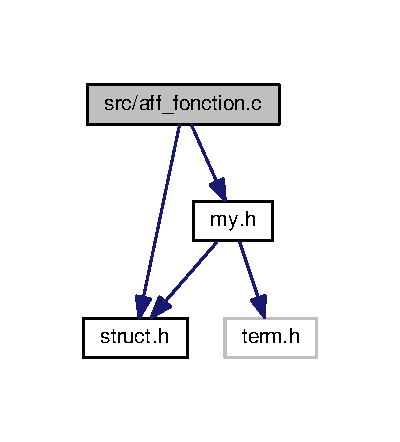
\includegraphics[width=192pt]{aff__fonction_8c__incl}
\end{center}
\end{figure}
\subsection*{Functions}
\begin{DoxyCompactItemize}
\item 
int \hyperlink{aff__fonction_8c_ad6bd0bdb80ac24e3e29cf46c10174da7}{my\+\_\+put\+\_\+selec} (\hyperlink{struct_8h_abb3da8aaebffbf4c0c44fc37b91a41af}{t\+\_\+eta} $\ast$etat)
\item 
void \hyperlink{aff__fonction_8c_a80713534eea50b2166e3a0cc23a9b331}{my\+\_\+aff\+\_\+underscor} (\hyperlink{struct_8h_abb3da8aaebffbf4c0c44fc37b91a41af}{t\+\_\+eta} $\ast$etat, int i, int size\+\_\+colone)
\item 
void \hyperlink{aff__fonction_8c_a5d95cd733d02a2d93e125f086528e2a4}{my\+\_\+aff\+\_\+select} (\hyperlink{struct_8h_abb3da8aaebffbf4c0c44fc37b91a41af}{t\+\_\+eta} $\ast$etat, int i, int size\+\_\+colone)
\item 
void \hyperlink{aff__fonction_8c_acb2ac8818ebb3c5e45bcc2017f5b7aab}{my\+\_\+aff\+\_\+under\+\_\+select} (\hyperlink{struct_8h_abb3da8aaebffbf4c0c44fc37b91a41af}{t\+\_\+eta} $\ast$etat, int i, int size\+\_\+colone)
\item 
int \hyperlink{aff__fonction_8c_a967439e4f4d08ca7783c0325fb74afed}{my\+\_\+aff\+\_\+fonc} (int i, int colone, \hyperlink{struct_8h_abb3da8aaebffbf4c0c44fc37b91a41af}{t\+\_\+eta} $\ast$etat, int size\+\_\+colone)
\end{DoxyCompactItemize}


\subsection{Function Documentation}
\hypertarget{aff__fonction_8c_a967439e4f4d08ca7783c0325fb74afed}{\index{aff\+\_\+fonction.\+c@{aff\+\_\+fonction.\+c}!my\+\_\+aff\+\_\+fonc@{my\+\_\+aff\+\_\+fonc}}
\index{my\+\_\+aff\+\_\+fonc@{my\+\_\+aff\+\_\+fonc}!aff\+\_\+fonction.\+c@{aff\+\_\+fonction.\+c}}
\subsubsection[{my\+\_\+aff\+\_\+fonc}]{\setlength{\rightskip}{0pt plus 5cm}int my\+\_\+aff\+\_\+fonc (
\begin{DoxyParamCaption}
\item[{int}]{i, }
\item[{int}]{colone, }
\item[{{\bf t\+\_\+eta} $\ast$}]{etat, }
\item[{int}]{size\+\_\+colone}
\end{DoxyParamCaption}
)}}\label{aff__fonction_8c_a967439e4f4d08ca7783c0325fb74afed}


Definition at line 55 of file aff\+\_\+fonction.\+c.

\hypertarget{aff__fonction_8c_a5d95cd733d02a2d93e125f086528e2a4}{\index{aff\+\_\+fonction.\+c@{aff\+\_\+fonction.\+c}!my\+\_\+aff\+\_\+select@{my\+\_\+aff\+\_\+select}}
\index{my\+\_\+aff\+\_\+select@{my\+\_\+aff\+\_\+select}!aff\+\_\+fonction.\+c@{aff\+\_\+fonction.\+c}}
\subsubsection[{my\+\_\+aff\+\_\+select}]{\setlength{\rightskip}{0pt plus 5cm}void my\+\_\+aff\+\_\+select (
\begin{DoxyParamCaption}
\item[{{\bf t\+\_\+eta} $\ast$}]{etat, }
\item[{int}]{i, }
\item[{int}]{size\+\_\+colone}
\end{DoxyParamCaption}
)}}\label{aff__fonction_8c_a5d95cd733d02a2d93e125f086528e2a4}


Definition at line 39 of file aff\+\_\+fonction.\+c.

\hypertarget{aff__fonction_8c_acb2ac8818ebb3c5e45bcc2017f5b7aab}{\index{aff\+\_\+fonction.\+c@{aff\+\_\+fonction.\+c}!my\+\_\+aff\+\_\+under\+\_\+select@{my\+\_\+aff\+\_\+under\+\_\+select}}
\index{my\+\_\+aff\+\_\+under\+\_\+select@{my\+\_\+aff\+\_\+under\+\_\+select}!aff\+\_\+fonction.\+c@{aff\+\_\+fonction.\+c}}
\subsubsection[{my\+\_\+aff\+\_\+under\+\_\+select}]{\setlength{\rightskip}{0pt plus 5cm}void my\+\_\+aff\+\_\+under\+\_\+select (
\begin{DoxyParamCaption}
\item[{{\bf t\+\_\+eta} $\ast$}]{etat, }
\item[{int}]{i, }
\item[{int}]{size\+\_\+colone}
\end{DoxyParamCaption}
)}}\label{aff__fonction_8c_acb2ac8818ebb3c5e45bcc2017f5b7aab}


Definition at line 47 of file aff\+\_\+fonction.\+c.

\hypertarget{aff__fonction_8c_a80713534eea50b2166e3a0cc23a9b331}{\index{aff\+\_\+fonction.\+c@{aff\+\_\+fonction.\+c}!my\+\_\+aff\+\_\+underscor@{my\+\_\+aff\+\_\+underscor}}
\index{my\+\_\+aff\+\_\+underscor@{my\+\_\+aff\+\_\+underscor}!aff\+\_\+fonction.\+c@{aff\+\_\+fonction.\+c}}
\subsubsection[{my\+\_\+aff\+\_\+underscor}]{\setlength{\rightskip}{0pt plus 5cm}void my\+\_\+aff\+\_\+underscor (
\begin{DoxyParamCaption}
\item[{{\bf t\+\_\+eta} $\ast$}]{etat, }
\item[{int}]{i, }
\item[{int}]{size\+\_\+colone}
\end{DoxyParamCaption}
)}}\label{aff__fonction_8c_a80713534eea50b2166e3a0cc23a9b331}


Definition at line 31 of file aff\+\_\+fonction.\+c.

\hypertarget{aff__fonction_8c_ad6bd0bdb80ac24e3e29cf46c10174da7}{\index{aff\+\_\+fonction.\+c@{aff\+\_\+fonction.\+c}!my\+\_\+put\+\_\+selec@{my\+\_\+put\+\_\+selec}}
\index{my\+\_\+put\+\_\+selec@{my\+\_\+put\+\_\+selec}!aff\+\_\+fonction.\+c@{aff\+\_\+fonction.\+c}}
\subsubsection[{my\+\_\+put\+\_\+selec}]{\setlength{\rightskip}{0pt plus 5cm}int my\+\_\+put\+\_\+selec (
\begin{DoxyParamCaption}
\item[{{\bf t\+\_\+eta} $\ast$}]{etat}
\end{DoxyParamCaption}
)}}\label{aff__fonction_8c_ad6bd0bdb80ac24e3e29cf46c10174da7}


Definition at line 14 of file aff\+\_\+fonction.\+c.


\hypertarget{main_8c}{\section{src/main.c File Reference}
\label{main_8c}\index{src/main.\+c@{src/main.\+c}}
}
{\ttfamily \#include $<$stdlib.\+h$>$}\\*
{\ttfamily \#include $<$sys/ioctl.\+h$>$}\\*
{\ttfamily \#include $<$termcap.\+h$>$}\\*
{\ttfamily \#include $<$term.\+h$>$}\\*
{\ttfamily \#include $<$ncurses/curses.\+h$>$}\\*
{\ttfamily \#include $<$termios.\+h$>$}\\*
{\ttfamily \#include $<$unistd.\+h$>$}\\*
{\ttfamily \#include $<$stdio.\+h$>$}\\*
{\ttfamily \#include $<$signal.\+h$>$}\\*
{\ttfamily \#include \char`\"{}struct.\+h\char`\"{}}\\*
{\ttfamily \#include \char`\"{}my.\+h\char`\"{}}\\*
Include dependency graph for main.\+c\+:\nopagebreak
\begin{figure}[H]
\begin{center}
\leavevmode
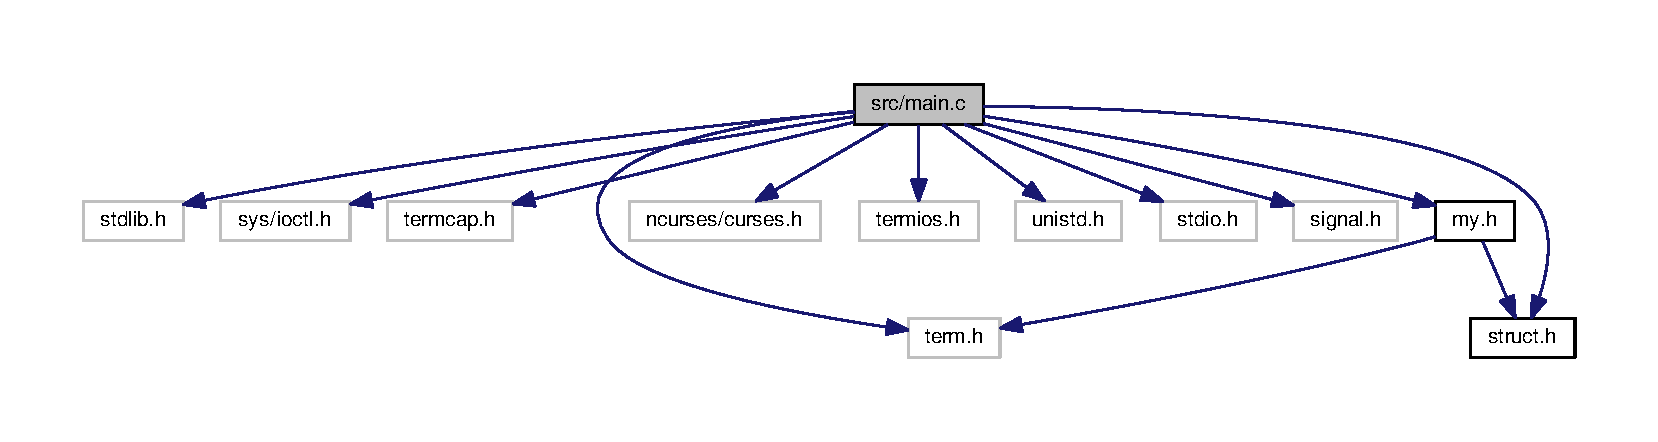
\includegraphics[width=350pt]{main_8c__incl}
\end{center}
\end{figure}
\subsection*{Functions}
\begin{DoxyCompactItemize}
\item 
int \hyperlink{main_8c_a3c04138a5bfe5d72780bb7e82a18e627}{main} (int argc, char $\ast$$\ast$argv)
\end{DoxyCompactItemize}


\subsection{Function Documentation}
\hypertarget{main_8c_a3c04138a5bfe5d72780bb7e82a18e627}{\index{main.\+c@{main.\+c}!main@{main}}
\index{main@{main}!main.\+c@{main.\+c}}
\subsubsection[{main}]{\setlength{\rightskip}{0pt plus 5cm}int main (
\begin{DoxyParamCaption}
\item[{int}]{argc, }
\item[{char $\ast$$\ast$}]{argv}
\end{DoxyParamCaption}
)}}\label{main_8c_a3c04138a5bfe5d72780bb7e82a18e627}


Definition at line 23 of file main.\+c.


\hypertarget{my_8h}{\section{src/my.h File Reference}
\label{my_8h}\index{src/my.\+h@{src/my.\+h}}
}
{\ttfamily \#include $<$term.\+h$>$}\\*
{\ttfamily \#include \char`\"{}struct.\+h\char`\"{}}\\*
Include dependency graph for my.\+h\+:\nopagebreak
\begin{figure}[H]
\begin{center}
\leavevmode
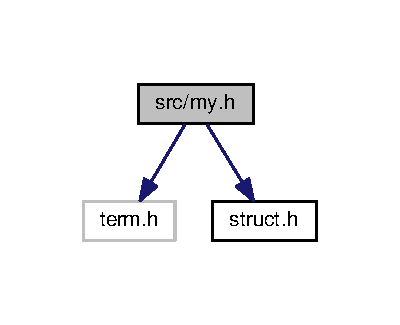
\includegraphics[width=192pt]{my_8h__incl}
\end{center}
\end{figure}
This graph shows which files directly or indirectly include this file\+:\nopagebreak
\begin{figure}[H]
\begin{center}
\leavevmode
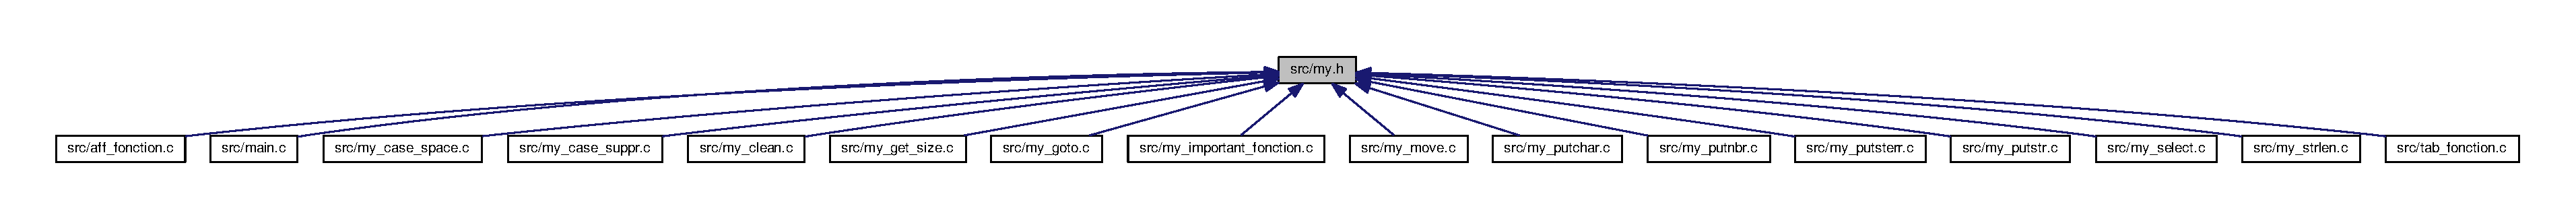
\includegraphics[width=350pt]{my_8h__dep__incl}
\end{center}
\end{figure}
\subsection*{Functions}
\begin{DoxyCompactItemize}
\item 
void \hyperlink{my_8h_ac4de74d04dc6e263345755eb62676802}{my\+\_\+putchar} (char c)
\item 
void \hyperlink{my_8h_a25366074e11e8eddaa1ba04a2ee13b55}{my\+\_\+putnbr} (int nb)
\item 
void \hyperlink{my_8h_a90745b48b1811f18086f358dc2b85fd4}{my\+\_\+putstr} (char $\ast$str)
\item 
void \hyperlink{my_8h_abbc8e0d57c6e21f89c3367ece5d6a5c6}{my\+\_\+putsterr} (char $\ast$str)
\item 
int \hyperlink{my_8h_a38fd644159c2b6ce04b987a9a9eb9eb5}{case\+\_\+right} (\hyperlink{struct_8h_abb3da8aaebffbf4c0c44fc37b91a41af}{t\+\_\+eta} $\ast$etat)
\item 
int \hyperlink{my_8h_a7ed81da7f401ef400973c6f141adac79}{case\+\_\+hight} (\hyperlink{struct_8h_abb3da8aaebffbf4c0c44fc37b91a41af}{t\+\_\+eta} $\ast$etat)
\item 
int \hyperlink{my_8h_a2451a5c10e20e4b4cb9e0d53bccfcd2a}{case\+\_\+down} (\hyperlink{struct_8h_abb3da8aaebffbf4c0c44fc37b91a41af}{t\+\_\+eta} $\ast$etat)
\item 
int \hyperlink{my_8h_af686d676ef6348cae9c7ce6de35b6223}{case\+\_\+left} (\hyperlink{struct_8h_abb3da8aaebffbf4c0c44fc37b91a41af}{t\+\_\+eta} $\ast$etat)
\item 
int \hyperlink{my_8h_ad41a2fc8dcc349d0cc3223eddba3d038}{my\+\_\+putc} (int c)
\item 
int \hyperlink{my_8h_a54107884475937a6a75a9cf11d24a4e2}{my\+\_\+actualisation} (struct termios $\ast$term)
\item 
void \hyperlink{my_8h_a72df070a1ab4704b8545b03005769b19}{my\+\_\+show\+\_\+tab} (\hyperlink{struct_8h_abb3da8aaebffbf4c0c44fc37b91a41af}{t\+\_\+eta} $\ast$etat, \hyperlink{struct_8h_a926b4cd56a88892e139db39d72aa5753}{t\+\_\+win} $\ast$win, int size\+\_\+colone)
\item 
void \hyperlink{my_8h_a88bfe7e43663ce4cbc564ab7a8a214fd}{my\+\_\+clean} (\hyperlink{struct_8h_a926b4cd56a88892e139db39d72aa5753}{t\+\_\+win} $\ast$win)
\item 
int \hyperlink{my_8h_add91d018cb04acdfb4a5512ca3b19e9d}{my\+\_\+select} (struct termios $\ast$term, \hyperlink{struct_8h_abb3da8aaebffbf4c0c44fc37b91a41af}{t\+\_\+eta} $\ast$etat, int size\+\_\+colone)
\item 
int \hyperlink{my_8h_aeaf66e886e7b245a2b3dece3103f2a66}{my\+\_\+ptr\+\_\+tab} (unsigned long buffer, \hyperlink{struct_8h_abb3da8aaebffbf4c0c44fc37b91a41af}{t\+\_\+eta} $\ast$etat)
\item 
int \hyperlink{my_8h_a7c31a994c5ec79ecf4144f4ef717112f}{my\+\_\+gere\+\_\+select} (int argc, char $\ast$$\ast$argv, int size\+\_\+colone, struct termios $\ast$term)
\item 
void \hyperlink{my_8h_a321389cb2b297d65458e3bc9b80b2410}{my\+\_\+putstr\+\_\+lime} (char $\ast$str, int lime)
\item 
int \hyperlink{my_8h_ad868f8855e4adc4512d7212c8705225a}{my\+\_\+gere\+\_\+key} (struct termios $\ast$term, \hyperlink{struct_8h_abb3da8aaebffbf4c0c44fc37b91a41af}{t\+\_\+eta} $\ast$etat)
\item 
int \hyperlink{my_8h_abcaef6165769ee9471db2e0db059f597}{case\+\_\+space} (\hyperlink{struct_8h_abb3da8aaebffbf4c0c44fc37b91a41af}{t\+\_\+eta} $\ast$etat)
\item 
void \hyperlink{my_8h_a07d17d9593512770b9c6c7d46a6ae5c7}{my\+\_\+put\+\_\+space} (int i)
\item 
int \hyperlink{my_8h_aab1aef2e8253b87e8d78436adf1b5de3}{case\+\_\+suppr} (\hyperlink{struct_8h_abb3da8aaebffbf4c0c44fc37b91a41af}{t\+\_\+eta} $\ast$etat)
\item 
void \hyperlink{my_8h_ab8c42cc361342e8e3e0e9ff5456ea431}{my\+\_\+putchar\+\_\+fd0} (char c)
\item 
void \hyperlink{my_8h_a4dd00910c0d38d20009f91c610e91ec7}{my\+\_\+putstr\+\_\+fd0} (char $\ast$str)
\item 
int \hyperlink{my_8h_ad6bd0bdb80ac24e3e29cf46c10174da7}{my\+\_\+put\+\_\+selec} (\hyperlink{struct_8h_abb3da8aaebffbf4c0c44fc37b91a41af}{t\+\_\+eta} $\ast$etat)
\item 
int \hyperlink{my_8h_a967439e4f4d08ca7783c0325fb74afed}{my\+\_\+aff\+\_\+fonc} (int i, int colone, \hyperlink{struct_8h_abb3da8aaebffbf4c0c44fc37b91a41af}{t\+\_\+eta} $\ast$etat, int size\+\_\+colone)
\item 
void \hyperlink{my_8h_a0b40897ed653fce4e3062e7adbd74e9e}{my\+\_\+aff\+\_\+underscore} (\hyperlink{struct_8h_abb3da8aaebffbf4c0c44fc37b91a41af}{t\+\_\+eta} $\ast$etat, int i, int size\+\_\+colone)
\item 
void \hyperlink{my_8h_a5d95cd733d02a2d93e125f086528e2a4}{my\+\_\+aff\+\_\+select} (\hyperlink{struct_8h_abb3da8aaebffbf4c0c44fc37b91a41af}{t\+\_\+eta} $\ast$etat, int i, int size\+\_\+colone)
\item 
void \hyperlink{my_8h_acb2ac8818ebb3c5e45bcc2017f5b7aab}{my\+\_\+aff\+\_\+under\+\_\+select} (\hyperlink{struct_8h_abb3da8aaebffbf4c0c44fc37b91a41af}{t\+\_\+eta} $\ast$etat, int i, int size\+\_\+colone)
\item 
int \hyperlink{my_8h_ac7e9bd08d068851e31a5b6d408004638}{my\+\_\+strlen} (char $\ast$str)
\item 
void \hyperlink{my_8h_a80713534eea50b2166e3a0cc23a9b331}{my\+\_\+aff\+\_\+underscor} (\hyperlink{struct_8h_abb3da8aaebffbf4c0c44fc37b91a41af}{t\+\_\+eta} $\ast$etat, int i, int size\+\_\+colone)
\item 
int \hyperlink{my_8h_a28a19d24f3bad205b4e78821a9b12c67}{get\+\_\+colone\+\_\+size} (int argc, char $\ast$$\ast$argv)
\item 
int \hyperlink{my_8h_a95d593084e9f262eea733689cf08e023}{nb\+\_\+colone} (int i, int colone, \hyperlink{struct_8h_a926b4cd56a88892e139db39d72aa5753}{t\+\_\+win} $\ast$win, \hyperlink{struct_8h_abb3da8aaebffbf4c0c44fc37b91a41af}{t\+\_\+eta} $\ast$etat)
\item 
void \hyperlink{my_8h_a91d6348b48c15f044abee99da6fec6bd}{nothing} ()
\item 
void \hyperlink{my_8h_ac787a46c22238927aeccb015549de725}{my\+\_\+init\+\_\+tab} (\hyperlink{struct_8h_abb3da8aaebffbf4c0c44fc37b91a41af}{t\+\_\+eta} $\ast$etat, int argc, char $\ast$$\ast$argv)
\item 
void \hyperlink{my_8h_ae57b39178fc6e120887784d5059ad877}{my\+\_\+alignement} (int i, int colone)
\item 
void \hyperlink{my_8h_a3345c21ddbb51ea1dedbec3ef94da186}{my\+\_\+err\+\_\+size} (int i, int colone, \hyperlink{struct_8h_a926b4cd56a88892e139db39d72aa5753}{t\+\_\+win} $\ast$win, int size\+\_\+colone)
\item 
int \hyperlink{my_8h_a350216f65167dc738d9ed40d460b8225}{my\+\_\+final\+\_\+clear} ()
\item 
int \hyperlink{my_8h_a28ba425582457bfcd22b6f82d2ce5566}{my\+\_\+put\+\_\+rest} (struct termios $\ast$term)
\end{DoxyCompactItemize}


\subsection{Function Documentation}
\hypertarget{my_8h_a2451a5c10e20e4b4cb9e0d53bccfcd2a}{\index{my.\+h@{my.\+h}!case\+\_\+down@{case\+\_\+down}}
\index{case\+\_\+down@{case\+\_\+down}!my.\+h@{my.\+h}}
\subsubsection[{case\+\_\+down}]{\setlength{\rightskip}{0pt plus 5cm}int case\+\_\+down (
\begin{DoxyParamCaption}
\item[{{\bf t\+\_\+eta} $\ast$}]{etat}
\end{DoxyParamCaption}
)}}\label{my_8h_a2451a5c10e20e4b4cb9e0d53bccfcd2a}


Definition at line 14 of file my\+\_\+move.\+c.

\hypertarget{my_8h_a7ed81da7f401ef400973c6f141adac79}{\index{my.\+h@{my.\+h}!case\+\_\+hight@{case\+\_\+hight}}
\index{case\+\_\+hight@{case\+\_\+hight}!my.\+h@{my.\+h}}
\subsubsection[{case\+\_\+hight}]{\setlength{\rightskip}{0pt plus 5cm}int case\+\_\+hight (
\begin{DoxyParamCaption}
\item[{{\bf t\+\_\+eta} $\ast$}]{etat}
\end{DoxyParamCaption}
)}}\label{my_8h_a7ed81da7f401ef400973c6f141adac79}


Definition at line 34 of file my\+\_\+move.\+c.

\hypertarget{my_8h_af686d676ef6348cae9c7ce6de35b6223}{\index{my.\+h@{my.\+h}!case\+\_\+left@{case\+\_\+left}}
\index{case\+\_\+left@{case\+\_\+left}!my.\+h@{my.\+h}}
\subsubsection[{case\+\_\+left}]{\setlength{\rightskip}{0pt plus 5cm}int case\+\_\+left (
\begin{DoxyParamCaption}
\item[{{\bf t\+\_\+eta} $\ast$}]{etat}
\end{DoxyParamCaption}
)}}\label{my_8h_af686d676ef6348cae9c7ce6de35b6223}


Definition at line 54 of file my\+\_\+move.\+c.

\hypertarget{my_8h_a38fd644159c2b6ce04b987a9a9eb9eb5}{\index{my.\+h@{my.\+h}!case\+\_\+right@{case\+\_\+right}}
\index{case\+\_\+right@{case\+\_\+right}!my.\+h@{my.\+h}}
\subsubsection[{case\+\_\+right}]{\setlength{\rightskip}{0pt plus 5cm}int case\+\_\+right (
\begin{DoxyParamCaption}
\item[{{\bf t\+\_\+eta} $\ast$}]{etat}
\end{DoxyParamCaption}
)}}\label{my_8h_a38fd644159c2b6ce04b987a9a9eb9eb5}


Definition at line 60 of file my\+\_\+move.\+c.

\hypertarget{my_8h_abcaef6165769ee9471db2e0db059f597}{\index{my.\+h@{my.\+h}!case\+\_\+space@{case\+\_\+space}}
\index{case\+\_\+space@{case\+\_\+space}!my.\+h@{my.\+h}}
\subsubsection[{case\+\_\+space}]{\setlength{\rightskip}{0pt plus 5cm}int case\+\_\+space (
\begin{DoxyParamCaption}
\item[{{\bf t\+\_\+eta} $\ast$}]{etat}
\end{DoxyParamCaption}
)}}\label{my_8h_abcaef6165769ee9471db2e0db059f597}


Definition at line 14 of file my\+\_\+case\+\_\+space.\+c.

\hypertarget{my_8h_aab1aef2e8253b87e8d78436adf1b5de3}{\index{my.\+h@{my.\+h}!case\+\_\+suppr@{case\+\_\+suppr}}
\index{case\+\_\+suppr@{case\+\_\+suppr}!my.\+h@{my.\+h}}
\subsubsection[{case\+\_\+suppr}]{\setlength{\rightskip}{0pt plus 5cm}int case\+\_\+suppr (
\begin{DoxyParamCaption}
\item[{{\bf t\+\_\+eta} $\ast$}]{etat}
\end{DoxyParamCaption}
)}}\label{my_8h_aab1aef2e8253b87e8d78436adf1b5de3}


Definition at line 14 of file my\+\_\+case\+\_\+suppr.\+c.

\hypertarget{my_8h_a28a19d24f3bad205b4e78821a9b12c67}{\index{my.\+h@{my.\+h}!get\+\_\+colone\+\_\+size@{get\+\_\+colone\+\_\+size}}
\index{get\+\_\+colone\+\_\+size@{get\+\_\+colone\+\_\+size}!my.\+h@{my.\+h}}
\subsubsection[{get\+\_\+colone\+\_\+size}]{\setlength{\rightskip}{0pt plus 5cm}int get\+\_\+colone\+\_\+size (
\begin{DoxyParamCaption}
\item[{int}]{argc, }
\item[{char $\ast$$\ast$}]{argv}
\end{DoxyParamCaption}
)}}\label{my_8h_a28a19d24f3bad205b4e78821a9b12c67}


Definition at line 25 of file my\+\_\+get\+\_\+size.\+c.

\hypertarget{my_8h_a54107884475937a6a75a9cf11d24a4e2}{\index{my.\+h@{my.\+h}!my\+\_\+actualisation@{my\+\_\+actualisation}}
\index{my\+\_\+actualisation@{my\+\_\+actualisation}!my.\+h@{my.\+h}}
\subsubsection[{my\+\_\+actualisation}]{\setlength{\rightskip}{0pt plus 5cm}int my\+\_\+actualisation (
\begin{DoxyParamCaption}
\item[{struct termios $\ast$}]{term}
\end{DoxyParamCaption}
)}}\label{my_8h_a54107884475937a6a75a9cf11d24a4e2}


Definition at line 21 of file my\+\_\+select.\+c.

\hypertarget{my_8h_a967439e4f4d08ca7783c0325fb74afed}{\index{my.\+h@{my.\+h}!my\+\_\+aff\+\_\+fonc@{my\+\_\+aff\+\_\+fonc}}
\index{my\+\_\+aff\+\_\+fonc@{my\+\_\+aff\+\_\+fonc}!my.\+h@{my.\+h}}
\subsubsection[{my\+\_\+aff\+\_\+fonc}]{\setlength{\rightskip}{0pt plus 5cm}int my\+\_\+aff\+\_\+fonc (
\begin{DoxyParamCaption}
\item[{int}]{i, }
\item[{int}]{colone, }
\item[{{\bf t\+\_\+eta} $\ast$}]{etat, }
\item[{int}]{size\+\_\+colone}
\end{DoxyParamCaption}
)}}\label{my_8h_a967439e4f4d08ca7783c0325fb74afed}


Definition at line 55 of file aff\+\_\+fonction.\+c.

\hypertarget{my_8h_a5d95cd733d02a2d93e125f086528e2a4}{\index{my.\+h@{my.\+h}!my\+\_\+aff\+\_\+select@{my\+\_\+aff\+\_\+select}}
\index{my\+\_\+aff\+\_\+select@{my\+\_\+aff\+\_\+select}!my.\+h@{my.\+h}}
\subsubsection[{my\+\_\+aff\+\_\+select}]{\setlength{\rightskip}{0pt plus 5cm}void my\+\_\+aff\+\_\+select (
\begin{DoxyParamCaption}
\item[{{\bf t\+\_\+eta} $\ast$}]{etat, }
\item[{int}]{i, }
\item[{int}]{size\+\_\+colone}
\end{DoxyParamCaption}
)}}\label{my_8h_a5d95cd733d02a2d93e125f086528e2a4}


Definition at line 39 of file aff\+\_\+fonction.\+c.

\hypertarget{my_8h_acb2ac8818ebb3c5e45bcc2017f5b7aab}{\index{my.\+h@{my.\+h}!my\+\_\+aff\+\_\+under\+\_\+select@{my\+\_\+aff\+\_\+under\+\_\+select}}
\index{my\+\_\+aff\+\_\+under\+\_\+select@{my\+\_\+aff\+\_\+under\+\_\+select}!my.\+h@{my.\+h}}
\subsubsection[{my\+\_\+aff\+\_\+under\+\_\+select}]{\setlength{\rightskip}{0pt plus 5cm}void my\+\_\+aff\+\_\+under\+\_\+select (
\begin{DoxyParamCaption}
\item[{{\bf t\+\_\+eta} $\ast$}]{etat, }
\item[{int}]{i, }
\item[{int}]{size\+\_\+colone}
\end{DoxyParamCaption}
)}}\label{my_8h_acb2ac8818ebb3c5e45bcc2017f5b7aab}


Definition at line 47 of file aff\+\_\+fonction.\+c.

\hypertarget{my_8h_a80713534eea50b2166e3a0cc23a9b331}{\index{my.\+h@{my.\+h}!my\+\_\+aff\+\_\+underscor@{my\+\_\+aff\+\_\+underscor}}
\index{my\+\_\+aff\+\_\+underscor@{my\+\_\+aff\+\_\+underscor}!my.\+h@{my.\+h}}
\subsubsection[{my\+\_\+aff\+\_\+underscor}]{\setlength{\rightskip}{0pt plus 5cm}void my\+\_\+aff\+\_\+underscor (
\begin{DoxyParamCaption}
\item[{{\bf t\+\_\+eta} $\ast$}]{etat, }
\item[{int}]{i, }
\item[{int}]{size\+\_\+colone}
\end{DoxyParamCaption}
)}}\label{my_8h_a80713534eea50b2166e3a0cc23a9b331}


Definition at line 31 of file aff\+\_\+fonction.\+c.

\hypertarget{my_8h_a0b40897ed653fce4e3062e7adbd74e9e}{\index{my.\+h@{my.\+h}!my\+\_\+aff\+\_\+underscore@{my\+\_\+aff\+\_\+underscore}}
\index{my\+\_\+aff\+\_\+underscore@{my\+\_\+aff\+\_\+underscore}!my.\+h@{my.\+h}}
\subsubsection[{my\+\_\+aff\+\_\+underscore}]{\setlength{\rightskip}{0pt plus 5cm}void my\+\_\+aff\+\_\+underscore (
\begin{DoxyParamCaption}
\item[{{\bf t\+\_\+eta} $\ast$}]{etat, }
\item[{int}]{i, }
\item[{int}]{size\+\_\+colone}
\end{DoxyParamCaption}
)}}\label{my_8h_a0b40897ed653fce4e3062e7adbd74e9e}
\hypertarget{my_8h_ae57b39178fc6e120887784d5059ad877}{\index{my.\+h@{my.\+h}!my\+\_\+alignement@{my\+\_\+alignement}}
\index{my\+\_\+alignement@{my\+\_\+alignement}!my.\+h@{my.\+h}}
\subsubsection[{my\+\_\+alignement}]{\setlength{\rightskip}{0pt plus 5cm}void my\+\_\+alignement (
\begin{DoxyParamCaption}
\item[{int}]{i, }
\item[{int}]{colone}
\end{DoxyParamCaption}
)}}\label{my_8h_ae57b39178fc6e120887784d5059ad877}


Definition at line 29 of file my\+\_\+goto.\+c.

\hypertarget{my_8h_a88bfe7e43663ce4cbc564ab7a8a214fd}{\index{my.\+h@{my.\+h}!my\+\_\+clean@{my\+\_\+clean}}
\index{my\+\_\+clean@{my\+\_\+clean}!my.\+h@{my.\+h}}
\subsubsection[{my\+\_\+clean}]{\setlength{\rightskip}{0pt plus 5cm}void my\+\_\+clean (
\begin{DoxyParamCaption}
\item[{{\bf t\+\_\+win} $\ast$}]{win}
\end{DoxyParamCaption}
)}}\label{my_8h_a88bfe7e43663ce4cbc564ab7a8a214fd}


Definition at line 40 of file my\+\_\+clean.\+c.

\hypertarget{my_8h_a3345c21ddbb51ea1dedbec3ef94da186}{\index{my.\+h@{my.\+h}!my\+\_\+err\+\_\+size@{my\+\_\+err\+\_\+size}}
\index{my\+\_\+err\+\_\+size@{my\+\_\+err\+\_\+size}!my.\+h@{my.\+h}}
\subsubsection[{my\+\_\+err\+\_\+size}]{\setlength{\rightskip}{0pt plus 5cm}void my\+\_\+err\+\_\+size (
\begin{DoxyParamCaption}
\item[{int}]{i, }
\item[{int}]{colone, }
\item[{{\bf t\+\_\+win} $\ast$}]{win, }
\item[{int}]{size\+\_\+colone}
\end{DoxyParamCaption}
)}}\label{my_8h_a3345c21ddbb51ea1dedbec3ef94da186}


Definition at line 18 of file my\+\_\+goto.\+c.

\hypertarget{my_8h_a350216f65167dc738d9ed40d460b8225}{\index{my.\+h@{my.\+h}!my\+\_\+final\+\_\+clear@{my\+\_\+final\+\_\+clear}}
\index{my\+\_\+final\+\_\+clear@{my\+\_\+final\+\_\+clear}!my.\+h@{my.\+h}}
\subsubsection[{my\+\_\+final\+\_\+clear}]{\setlength{\rightskip}{0pt plus 5cm}int my\+\_\+final\+\_\+clear (
\begin{DoxyParamCaption}
{}
\end{DoxyParamCaption}
)}}\label{my_8h_a350216f65167dc738d9ed40d460b8225}


Definition at line 28 of file my\+\_\+clean.\+c.

\hypertarget{my_8h_ad868f8855e4adc4512d7212c8705225a}{\index{my.\+h@{my.\+h}!my\+\_\+gere\+\_\+key@{my\+\_\+gere\+\_\+key}}
\index{my\+\_\+gere\+\_\+key@{my\+\_\+gere\+\_\+key}!my.\+h@{my.\+h}}
\subsubsection[{my\+\_\+gere\+\_\+key}]{\setlength{\rightskip}{0pt plus 5cm}int my\+\_\+gere\+\_\+key (
\begin{DoxyParamCaption}
\item[{struct termios $\ast$}]{term, }
\item[{{\bf t\+\_\+eta} $\ast$}]{etat}
\end{DoxyParamCaption}
)}}\label{my_8h_ad868f8855e4adc4512d7212c8705225a}


Definition at line 56 of file my\+\_\+select.\+c.

\hypertarget{my_8h_a7c31a994c5ec79ecf4144f4ef717112f}{\index{my.\+h@{my.\+h}!my\+\_\+gere\+\_\+select@{my\+\_\+gere\+\_\+select}}
\index{my\+\_\+gere\+\_\+select@{my\+\_\+gere\+\_\+select}!my.\+h@{my.\+h}}
\subsubsection[{my\+\_\+gere\+\_\+select}]{\setlength{\rightskip}{0pt plus 5cm}int my\+\_\+gere\+\_\+select (
\begin{DoxyParamCaption}
\item[{int}]{argc, }
\item[{char $\ast$$\ast$}]{argv, }
\item[{int}]{size\+\_\+colone, }
\item[{struct termios $\ast$}]{term}
\end{DoxyParamCaption}
)}}\label{my_8h_a7c31a994c5ec79ecf4144f4ef717112f}


Definition at line 80 of file my\+\_\+select.\+c.

\hypertarget{my_8h_ac787a46c22238927aeccb015549de725}{\index{my.\+h@{my.\+h}!my\+\_\+init\+\_\+tab@{my\+\_\+init\+\_\+tab}}
\index{my\+\_\+init\+\_\+tab@{my\+\_\+init\+\_\+tab}!my.\+h@{my.\+h}}
\subsubsection[{my\+\_\+init\+\_\+tab}]{\setlength{\rightskip}{0pt plus 5cm}void my\+\_\+init\+\_\+tab (
\begin{DoxyParamCaption}
\item[{{\bf t\+\_\+eta} $\ast$}]{etat, }
\item[{int}]{argc, }
\item[{char $\ast$$\ast$}]{argv}
\end{DoxyParamCaption}
)}}\label{my_8h_ac787a46c22238927aeccb015549de725}


Definition at line 14 of file tab\+\_\+fonction.\+c.

\hypertarget{my_8h_aeaf66e886e7b245a2b3dece3103f2a66}{\index{my.\+h@{my.\+h}!my\+\_\+ptr\+\_\+tab@{my\+\_\+ptr\+\_\+tab}}
\index{my\+\_\+ptr\+\_\+tab@{my\+\_\+ptr\+\_\+tab}!my.\+h@{my.\+h}}
\subsubsection[{my\+\_\+ptr\+\_\+tab}]{\setlength{\rightskip}{0pt plus 5cm}int my\+\_\+ptr\+\_\+tab (
\begin{DoxyParamCaption}
\item[{unsigned long}]{buffer, }
\item[{{\bf t\+\_\+eta} $\ast$}]{etat}
\end{DoxyParamCaption}
)}}\label{my_8h_aeaf66e886e7b245a2b3dece3103f2a66}


Definition at line 33 of file tab\+\_\+fonction.\+c.

\hypertarget{my_8h_a28ba425582457bfcd22b6f82d2ce5566}{\index{my.\+h@{my.\+h}!my\+\_\+put\+\_\+rest@{my\+\_\+put\+\_\+rest}}
\index{my\+\_\+put\+\_\+rest@{my\+\_\+put\+\_\+rest}!my.\+h@{my.\+h}}
\subsubsection[{my\+\_\+put\+\_\+rest}]{\setlength{\rightskip}{0pt plus 5cm}int my\+\_\+put\+\_\+rest (
\begin{DoxyParamCaption}
\item[{struct termios $\ast$}]{term}
\end{DoxyParamCaption}
)}}\label{my_8h_a28ba425582457bfcd22b6f82d2ce5566}


Definition at line 18 of file my\+\_\+clean.\+c.

\hypertarget{my_8h_ad6bd0bdb80ac24e3e29cf46c10174da7}{\index{my.\+h@{my.\+h}!my\+\_\+put\+\_\+selec@{my\+\_\+put\+\_\+selec}}
\index{my\+\_\+put\+\_\+selec@{my\+\_\+put\+\_\+selec}!my.\+h@{my.\+h}}
\subsubsection[{my\+\_\+put\+\_\+selec}]{\setlength{\rightskip}{0pt plus 5cm}int my\+\_\+put\+\_\+selec (
\begin{DoxyParamCaption}
\item[{{\bf t\+\_\+eta} $\ast$}]{etat}
\end{DoxyParamCaption}
)}}\label{my_8h_ad6bd0bdb80ac24e3e29cf46c10174da7}


Definition at line 14 of file aff\+\_\+fonction.\+c.

\hypertarget{my_8h_a07d17d9593512770b9c6c7d46a6ae5c7}{\index{my.\+h@{my.\+h}!my\+\_\+put\+\_\+space@{my\+\_\+put\+\_\+space}}
\index{my\+\_\+put\+\_\+space@{my\+\_\+put\+\_\+space}!my.\+h@{my.\+h}}
\subsubsection[{my\+\_\+put\+\_\+space}]{\setlength{\rightskip}{0pt plus 5cm}void my\+\_\+put\+\_\+space (
\begin{DoxyParamCaption}
\item[{int}]{i}
\end{DoxyParamCaption}
)}}\label{my_8h_a07d17d9593512770b9c6c7d46a6ae5c7}


Definition at line 55 of file my\+\_\+putstr.\+c.

\hypertarget{my_8h_ad41a2fc8dcc349d0cc3223eddba3d038}{\index{my.\+h@{my.\+h}!my\+\_\+putc@{my\+\_\+putc}}
\index{my\+\_\+putc@{my\+\_\+putc}!my.\+h@{my.\+h}}
\subsubsection[{my\+\_\+putc}]{\setlength{\rightskip}{0pt plus 5cm}int my\+\_\+putc (
\begin{DoxyParamCaption}
\item[{int}]{c}
\end{DoxyParamCaption}
)}}\label{my_8h_ad41a2fc8dcc349d0cc3223eddba3d038}


Definition at line 24 of file my\+\_\+putchar.\+c.

\hypertarget{my_8h_ac4de74d04dc6e263345755eb62676802}{\index{my.\+h@{my.\+h}!my\+\_\+putchar@{my\+\_\+putchar}}
\index{my\+\_\+putchar@{my\+\_\+putchar}!my.\+h@{my.\+h}}
\subsubsection[{my\+\_\+putchar}]{\setlength{\rightskip}{0pt plus 5cm}void my\+\_\+putchar (
\begin{DoxyParamCaption}
\item[{char}]{c}
\end{DoxyParamCaption}
)}}\label{my_8h_ac4de74d04dc6e263345755eb62676802}


Definition at line 14 of file my\+\_\+putchar.\+c.

\hypertarget{my_8h_ab8c42cc361342e8e3e0e9ff5456ea431}{\index{my.\+h@{my.\+h}!my\+\_\+putchar\+\_\+fd0@{my\+\_\+putchar\+\_\+fd0}}
\index{my\+\_\+putchar\+\_\+fd0@{my\+\_\+putchar\+\_\+fd0}!my.\+h@{my.\+h}}
\subsubsection[{my\+\_\+putchar\+\_\+fd0}]{\setlength{\rightskip}{0pt plus 5cm}void my\+\_\+putchar\+\_\+fd0 (
\begin{DoxyParamCaption}
\item[{char}]{c}
\end{DoxyParamCaption}
)}}\label{my_8h_ab8c42cc361342e8e3e0e9ff5456ea431}


Definition at line 19 of file my\+\_\+putchar.\+c.

\hypertarget{my_8h_a25366074e11e8eddaa1ba04a2ee13b55}{\index{my.\+h@{my.\+h}!my\+\_\+putnbr@{my\+\_\+putnbr}}
\index{my\+\_\+putnbr@{my\+\_\+putnbr}!my.\+h@{my.\+h}}
\subsubsection[{my\+\_\+putnbr}]{\setlength{\rightskip}{0pt plus 5cm}void my\+\_\+putnbr (
\begin{DoxyParamCaption}
\item[{int}]{nb}
\end{DoxyParamCaption}
)}}\label{my_8h_a25366074e11e8eddaa1ba04a2ee13b55}


Definition at line 13 of file my\+\_\+putnbr.\+c.

\hypertarget{my_8h_abbc8e0d57c6e21f89c3367ece5d6a5c6}{\index{my.\+h@{my.\+h}!my\+\_\+putsterr@{my\+\_\+putsterr}}
\index{my\+\_\+putsterr@{my\+\_\+putsterr}!my.\+h@{my.\+h}}
\subsubsection[{my\+\_\+putsterr}]{\setlength{\rightskip}{0pt plus 5cm}void my\+\_\+putsterr (
\begin{DoxyParamCaption}
\item[{char $\ast$}]{str}
\end{DoxyParamCaption}
)}}\label{my_8h_abbc8e0d57c6e21f89c3367ece5d6a5c6}


Definition at line 20 of file my\+\_\+putsterr.\+c.

\hypertarget{my_8h_a90745b48b1811f18086f358dc2b85fd4}{\index{my.\+h@{my.\+h}!my\+\_\+putstr@{my\+\_\+putstr}}
\index{my\+\_\+putstr@{my\+\_\+putstr}!my.\+h@{my.\+h}}
\subsubsection[{my\+\_\+putstr}]{\setlength{\rightskip}{0pt plus 5cm}void my\+\_\+putstr (
\begin{DoxyParamCaption}
\item[{char $\ast$}]{str}
\end{DoxyParamCaption}
)}}\label{my_8h_a90745b48b1811f18086f358dc2b85fd4}


Definition at line 14 of file my\+\_\+putstr.\+c.

\hypertarget{my_8h_a4dd00910c0d38d20009f91c610e91ec7}{\index{my.\+h@{my.\+h}!my\+\_\+putstr\+\_\+fd0@{my\+\_\+putstr\+\_\+fd0}}
\index{my\+\_\+putstr\+\_\+fd0@{my\+\_\+putstr\+\_\+fd0}!my.\+h@{my.\+h}}
\subsubsection[{my\+\_\+putstr\+\_\+fd0}]{\setlength{\rightskip}{0pt plus 5cm}void my\+\_\+putstr\+\_\+fd0 (
\begin{DoxyParamCaption}
\item[{char $\ast$}]{str}
\end{DoxyParamCaption}
)}}\label{my_8h_a4dd00910c0d38d20009f91c610e91ec7}


Definition at line 26 of file my\+\_\+putstr.\+c.

\hypertarget{my_8h_a321389cb2b297d65458e3bc9b80b2410}{\index{my.\+h@{my.\+h}!my\+\_\+putstr\+\_\+lime@{my\+\_\+putstr\+\_\+lime}}
\index{my\+\_\+putstr\+\_\+lime@{my\+\_\+putstr\+\_\+lime}!my.\+h@{my.\+h}}
\subsubsection[{my\+\_\+putstr\+\_\+lime}]{\setlength{\rightskip}{0pt plus 5cm}void my\+\_\+putstr\+\_\+lime (
\begin{DoxyParamCaption}
\item[{char $\ast$}]{str, }
\item[{int}]{lime}
\end{DoxyParamCaption}
)}}\label{my_8h_a321389cb2b297d65458e3bc9b80b2410}


Definition at line 38 of file my\+\_\+putstr.\+c.

\hypertarget{my_8h_add91d018cb04acdfb4a5512ca3b19e9d}{\index{my.\+h@{my.\+h}!my\+\_\+select@{my\+\_\+select}}
\index{my\+\_\+select@{my\+\_\+select}!my.\+h@{my.\+h}}
\subsubsection[{my\+\_\+select}]{\setlength{\rightskip}{0pt plus 5cm}int my\+\_\+select (
\begin{DoxyParamCaption}
\item[{struct termios $\ast$}]{term, }
\item[{{\bf t\+\_\+eta} $\ast$}]{etat, }
\item[{int}]{size\+\_\+colone}
\end{DoxyParamCaption}
)}}\label{my_8h_add91d018cb04acdfb4a5512ca3b19e9d}


Definition at line 31 of file my\+\_\+select.\+c.

\hypertarget{my_8h_a72df070a1ab4704b8545b03005769b19}{\index{my.\+h@{my.\+h}!my\+\_\+show\+\_\+tab@{my\+\_\+show\+\_\+tab}}
\index{my\+\_\+show\+\_\+tab@{my\+\_\+show\+\_\+tab}!my.\+h@{my.\+h}}
\subsubsection[{my\+\_\+show\+\_\+tab}]{\setlength{\rightskip}{0pt plus 5cm}void my\+\_\+show\+\_\+tab (
\begin{DoxyParamCaption}
\item[{{\bf t\+\_\+eta} $\ast$}]{etat, }
\item[{{\bf t\+\_\+win} $\ast$}]{win, }
\item[{int}]{size\+\_\+colone}
\end{DoxyParamCaption}
)}}\label{my_8h_a72df070a1ab4704b8545b03005769b19}


Definition at line 54 of file tab\+\_\+fonction.\+c.

\hypertarget{my_8h_ac7e9bd08d068851e31a5b6d408004638}{\index{my.\+h@{my.\+h}!my\+\_\+strlen@{my\+\_\+strlen}}
\index{my\+\_\+strlen@{my\+\_\+strlen}!my.\+h@{my.\+h}}
\subsubsection[{my\+\_\+strlen}]{\setlength{\rightskip}{0pt plus 5cm}int my\+\_\+strlen (
\begin{DoxyParamCaption}
\item[{char $\ast$}]{str}
\end{DoxyParamCaption}
)}}\label{my_8h_ac7e9bd08d068851e31a5b6d408004638}


Definition at line 13 of file my\+\_\+strlen.\+c.

\hypertarget{my_8h_a95d593084e9f262eea733689cf08e023}{\index{my.\+h@{my.\+h}!nb\+\_\+colone@{nb\+\_\+colone}}
\index{nb\+\_\+colone@{nb\+\_\+colone}!my.\+h@{my.\+h}}
\subsubsection[{nb\+\_\+colone}]{\setlength{\rightskip}{0pt plus 5cm}int nb\+\_\+colone (
\begin{DoxyParamCaption}
\item[{int}]{i, }
\item[{int}]{colone, }
\item[{{\bf t\+\_\+win} $\ast$}]{win, }
\item[{{\bf t\+\_\+eta} $\ast$}]{etat}
\end{DoxyParamCaption}
)}}\label{my_8h_a95d593084e9f262eea733689cf08e023}


Definition at line 13 of file my\+\_\+get\+\_\+size.\+c.

\hypertarget{my_8h_a91d6348b48c15f044abee99da6fec6bd}{\index{my.\+h@{my.\+h}!nothing@{nothing}}
\index{nothing@{nothing}!my.\+h@{my.\+h}}
\subsubsection[{nothing}]{\setlength{\rightskip}{0pt plus 5cm}void nothing (
\begin{DoxyParamCaption}
{}
\end{DoxyParamCaption}
)}}\label{my_8h_a91d6348b48c15f044abee99da6fec6bd}


Definition at line 13 of file my\+\_\+important\+\_\+fonction.\+c.


\hypertarget{my__case__space_8c}{\section{src/my\+\_\+case\+\_\+space.c File Reference}
\label{my__case__space_8c}\index{src/my\+\_\+case\+\_\+space.\+c@{src/my\+\_\+case\+\_\+space.\+c}}
}
{\ttfamily \#include \char`\"{}struct.\+h\char`\"{}}\\*
{\ttfamily \#include \char`\"{}my.\+h\char`\"{}}\\*
Include dependency graph for my\+\_\+case\+\_\+space.\+c\+:\nopagebreak
\begin{figure}[H]
\begin{center}
\leavevmode
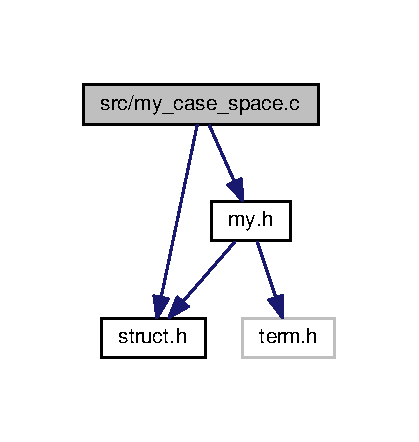
\includegraphics[width=201pt]{my__case__space_8c__incl}
\end{center}
\end{figure}
\subsection*{Functions}
\begin{DoxyCompactItemize}
\item 
int \hyperlink{my__case__space_8c_abcaef6165769ee9471db2e0db059f597}{case\+\_\+space} (\hyperlink{struct_8h_abb3da8aaebffbf4c0c44fc37b91a41af}{t\+\_\+eta} $\ast$etat)
\end{DoxyCompactItemize}


\subsection{Function Documentation}
\hypertarget{my__case__space_8c_abcaef6165769ee9471db2e0db059f597}{\index{my\+\_\+case\+\_\+space.\+c@{my\+\_\+case\+\_\+space.\+c}!case\+\_\+space@{case\+\_\+space}}
\index{case\+\_\+space@{case\+\_\+space}!my\+\_\+case\+\_\+space.\+c@{my\+\_\+case\+\_\+space.\+c}}
\subsubsection[{case\+\_\+space}]{\setlength{\rightskip}{0pt plus 5cm}int case\+\_\+space (
\begin{DoxyParamCaption}
\item[{{\bf t\+\_\+eta} $\ast$}]{etat}
\end{DoxyParamCaption}
)}}\label{my__case__space_8c_abcaef6165769ee9471db2e0db059f597}


Definition at line 14 of file my\+\_\+case\+\_\+space.\+c.


\hypertarget{my__case__suppr_8c}{\section{src/my\+\_\+case\+\_\+suppr.c File Reference}
\label{my__case__suppr_8c}\index{src/my\+\_\+case\+\_\+suppr.\+c@{src/my\+\_\+case\+\_\+suppr.\+c}}
}
{\ttfamily \#include \char`\"{}my.\+h\char`\"{}}\\*
{\ttfamily \#include \char`\"{}struct.\+h\char`\"{}}\\*
Include dependency graph for my\+\_\+case\+\_\+suppr.\+c\+:\nopagebreak
\begin{figure}[H]
\begin{center}
\leavevmode
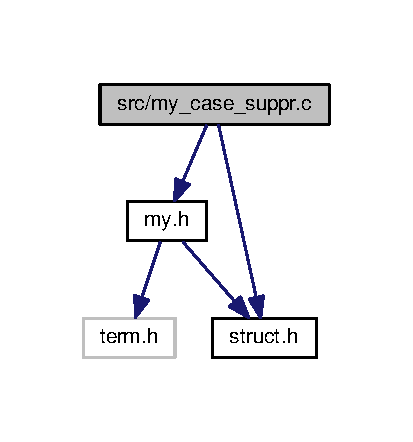
\includegraphics[width=198pt]{my__case__suppr_8c__incl}
\end{center}
\end{figure}
\subsection*{Functions}
\begin{DoxyCompactItemize}
\item 
int \hyperlink{my__case__suppr_8c_aab1aef2e8253b87e8d78436adf1b5de3}{case\+\_\+suppr} (\hyperlink{struct_8h_abb3da8aaebffbf4c0c44fc37b91a41af}{t\+\_\+eta} $\ast$etat)
\end{DoxyCompactItemize}


\subsection{Function Documentation}
\hypertarget{my__case__suppr_8c_aab1aef2e8253b87e8d78436adf1b5de3}{\index{my\+\_\+case\+\_\+suppr.\+c@{my\+\_\+case\+\_\+suppr.\+c}!case\+\_\+suppr@{case\+\_\+suppr}}
\index{case\+\_\+suppr@{case\+\_\+suppr}!my\+\_\+case\+\_\+suppr.\+c@{my\+\_\+case\+\_\+suppr.\+c}}
\subsubsection[{case\+\_\+suppr}]{\setlength{\rightskip}{0pt plus 5cm}int case\+\_\+suppr (
\begin{DoxyParamCaption}
\item[{{\bf t\+\_\+eta} $\ast$}]{etat}
\end{DoxyParamCaption}
)}}\label{my__case__suppr_8c_aab1aef2e8253b87e8d78436adf1b5de3}


Definition at line 14 of file my\+\_\+case\+\_\+suppr.\+c.


\hypertarget{my__clean_8c}{\section{src/my\+\_\+clean.c File Reference}
\label{my__clean_8c}\index{src/my\+\_\+clean.\+c@{src/my\+\_\+clean.\+c}}
}
{\ttfamily \#include $<$stdlib.\+h$>$}\\*
{\ttfamily \#include $<$sys/ioctl.\+h$>$}\\*
{\ttfamily \#include $<$termios.\+h$>$}\\*
{\ttfamily \#include $<$unistd.\+h$>$}\\*
{\ttfamily \#include \char`\"{}my.\+h\char`\"{}}\\*
{\ttfamily \#include \char`\"{}struct.\+h\char`\"{}}\\*
Include dependency graph for my\+\_\+clean.\+c\+:\nopagebreak
\begin{figure}[H]
\begin{center}
\leavevmode
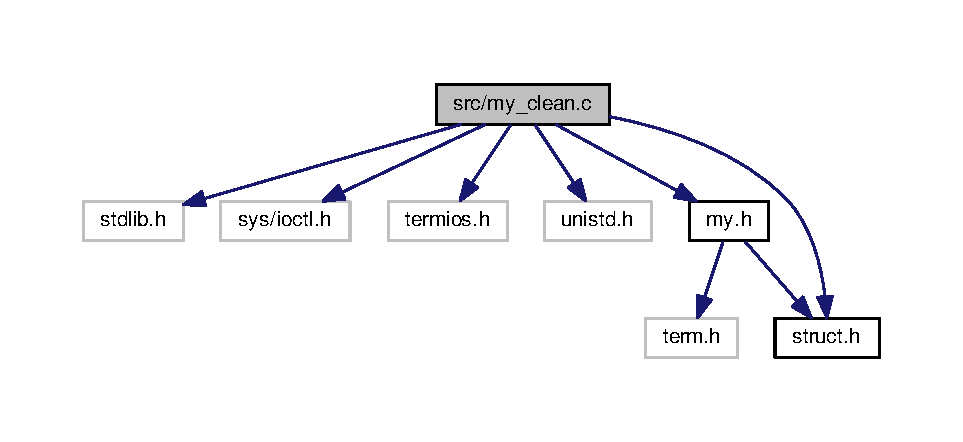
\includegraphics[width=350pt]{my__clean_8c__incl}
\end{center}
\end{figure}
\subsection*{Functions}
\begin{DoxyCompactItemize}
\item 
int \hyperlink{my__clean_8c_a28ba425582457bfcd22b6f82d2ce5566}{my\+\_\+put\+\_\+rest} (struct termios $\ast$term)
\item 
int \hyperlink{my__clean_8c_a350216f65167dc738d9ed40d460b8225}{my\+\_\+final\+\_\+clear} ()
\item 
void \hyperlink{my__clean_8c_a88bfe7e43663ce4cbc564ab7a8a214fd}{my\+\_\+clean} (\hyperlink{struct_8h_a926b4cd56a88892e139db39d72aa5753}{t\+\_\+win} $\ast$win)
\end{DoxyCompactItemize}


\subsection{Function Documentation}
\hypertarget{my__clean_8c_a88bfe7e43663ce4cbc564ab7a8a214fd}{\index{my\+\_\+clean.\+c@{my\+\_\+clean.\+c}!my\+\_\+clean@{my\+\_\+clean}}
\index{my\+\_\+clean@{my\+\_\+clean}!my\+\_\+clean.\+c@{my\+\_\+clean.\+c}}
\subsubsection[{my\+\_\+clean}]{\setlength{\rightskip}{0pt plus 5cm}void my\+\_\+clean (
\begin{DoxyParamCaption}
\item[{{\bf t\+\_\+win} $\ast$}]{win}
\end{DoxyParamCaption}
)}}\label{my__clean_8c_a88bfe7e43663ce4cbc564ab7a8a214fd}


Definition at line 40 of file my\+\_\+clean.\+c.

\hypertarget{my__clean_8c_a350216f65167dc738d9ed40d460b8225}{\index{my\+\_\+clean.\+c@{my\+\_\+clean.\+c}!my\+\_\+final\+\_\+clear@{my\+\_\+final\+\_\+clear}}
\index{my\+\_\+final\+\_\+clear@{my\+\_\+final\+\_\+clear}!my\+\_\+clean.\+c@{my\+\_\+clean.\+c}}
\subsubsection[{my\+\_\+final\+\_\+clear}]{\setlength{\rightskip}{0pt plus 5cm}int my\+\_\+final\+\_\+clear (
\begin{DoxyParamCaption}
{}
\end{DoxyParamCaption}
)}}\label{my__clean_8c_a350216f65167dc738d9ed40d460b8225}


Definition at line 28 of file my\+\_\+clean.\+c.

\hypertarget{my__clean_8c_a28ba425582457bfcd22b6f82d2ce5566}{\index{my\+\_\+clean.\+c@{my\+\_\+clean.\+c}!my\+\_\+put\+\_\+rest@{my\+\_\+put\+\_\+rest}}
\index{my\+\_\+put\+\_\+rest@{my\+\_\+put\+\_\+rest}!my\+\_\+clean.\+c@{my\+\_\+clean.\+c}}
\subsubsection[{my\+\_\+put\+\_\+rest}]{\setlength{\rightskip}{0pt plus 5cm}int my\+\_\+put\+\_\+rest (
\begin{DoxyParamCaption}
\item[{struct termios $\ast$}]{term}
\end{DoxyParamCaption}
)}}\label{my__clean_8c_a28ba425582457bfcd22b6f82d2ce5566}


Definition at line 18 of file my\+\_\+clean.\+c.


\hypertarget{my__get__size_8c}{\section{src/my\+\_\+get\+\_\+size.c File Reference}
\label{my__get__size_8c}\index{src/my\+\_\+get\+\_\+size.\+c@{src/my\+\_\+get\+\_\+size.\+c}}
}
{\ttfamily \#include \char`\"{}my.\+h\char`\"{}}\\*
Include dependency graph for my\+\_\+get\+\_\+size.\+c\+:\nopagebreak
\begin{figure}[H]
\begin{center}
\leavevmode
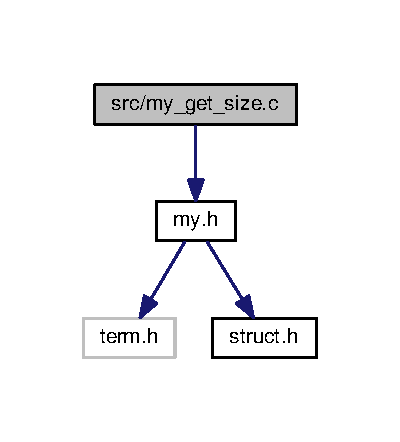
\includegraphics[width=192pt]{my__get__size_8c__incl}
\end{center}
\end{figure}
\subsection*{Functions}
\begin{DoxyCompactItemize}
\item 
int \hyperlink{my__get__size_8c_a95d593084e9f262eea733689cf08e023}{nb\+\_\+colone} (int i, int colone, \hyperlink{struct_8h_a926b4cd56a88892e139db39d72aa5753}{t\+\_\+win} $\ast$win, \hyperlink{struct_8h_abb3da8aaebffbf4c0c44fc37b91a41af}{t\+\_\+eta} $\ast$etat)
\item 
int \hyperlink{my__get__size_8c_a28a19d24f3bad205b4e78821a9b12c67}{get\+\_\+colone\+\_\+size} (int argc, char $\ast$$\ast$argv)
\end{DoxyCompactItemize}


\subsection{Function Documentation}
\hypertarget{my__get__size_8c_a28a19d24f3bad205b4e78821a9b12c67}{\index{my\+\_\+get\+\_\+size.\+c@{my\+\_\+get\+\_\+size.\+c}!get\+\_\+colone\+\_\+size@{get\+\_\+colone\+\_\+size}}
\index{get\+\_\+colone\+\_\+size@{get\+\_\+colone\+\_\+size}!my\+\_\+get\+\_\+size.\+c@{my\+\_\+get\+\_\+size.\+c}}
\subsubsection[{get\+\_\+colone\+\_\+size}]{\setlength{\rightskip}{0pt plus 5cm}int get\+\_\+colone\+\_\+size (
\begin{DoxyParamCaption}
\item[{int}]{argc, }
\item[{char $\ast$$\ast$}]{argv}
\end{DoxyParamCaption}
)}}\label{my__get__size_8c_a28a19d24f3bad205b4e78821a9b12c67}


Definition at line 25 of file my\+\_\+get\+\_\+size.\+c.

\hypertarget{my__get__size_8c_a95d593084e9f262eea733689cf08e023}{\index{my\+\_\+get\+\_\+size.\+c@{my\+\_\+get\+\_\+size.\+c}!nb\+\_\+colone@{nb\+\_\+colone}}
\index{nb\+\_\+colone@{nb\+\_\+colone}!my\+\_\+get\+\_\+size.\+c@{my\+\_\+get\+\_\+size.\+c}}
\subsubsection[{nb\+\_\+colone}]{\setlength{\rightskip}{0pt plus 5cm}int nb\+\_\+colone (
\begin{DoxyParamCaption}
\item[{int}]{i, }
\item[{int}]{colone, }
\item[{{\bf t\+\_\+win} $\ast$}]{win, }
\item[{{\bf t\+\_\+eta} $\ast$}]{etat}
\end{DoxyParamCaption}
)}}\label{my__get__size_8c_a95d593084e9f262eea733689cf08e023}


Definition at line 13 of file my\+\_\+get\+\_\+size.\+c.


\hypertarget{my__goto_8c}{\section{src/my\+\_\+goto.c File Reference}
\label{my__goto_8c}\index{src/my\+\_\+goto.\+c@{src/my\+\_\+goto.\+c}}
}
{\ttfamily \#include $<$stdlib.\+h$>$}\\*
{\ttfamily \#include $<$termcap.\+h$>$}\\*
{\ttfamily \#include $<$ncurses/curses.\+h$>$}\\*
{\ttfamily \#include $<$termios.\+h$>$}\\*
{\ttfamily \#include \char`\"{}struct.\+h\char`\"{}}\\*
{\ttfamily \#include \char`\"{}my.\+h\char`\"{}}\\*
Include dependency graph for my\+\_\+goto.\+c\+:\nopagebreak
\begin{figure}[H]
\begin{center}
\leavevmode
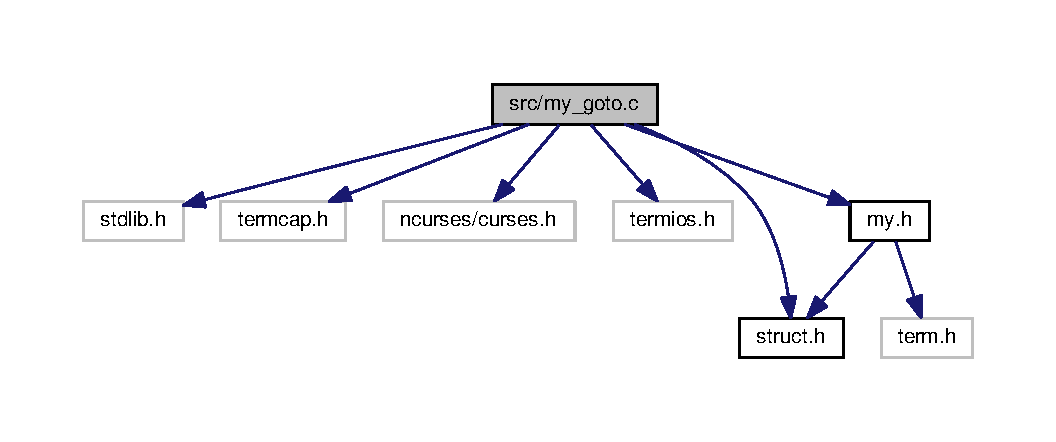
\includegraphics[width=350pt]{my__goto_8c__incl}
\end{center}
\end{figure}
\subsection*{Functions}
\begin{DoxyCompactItemize}
\item 
void \hyperlink{my__goto_8c_adea18f8771026f84b0928d239ecfc3c6}{my\+\_\+err\+\_\+size} (int i, int colone, \hyperlink{struct_8h_a926b4cd56a88892e139db39d72aa5753}{t\+\_\+win} $\ast$win, int size\+\_\+line)
\item 
void \hyperlink{my__goto_8c_ae57b39178fc6e120887784d5059ad877}{my\+\_\+alignement} (int i, int colone)
\end{DoxyCompactItemize}


\subsection{Function Documentation}
\hypertarget{my__goto_8c_ae57b39178fc6e120887784d5059ad877}{\index{my\+\_\+goto.\+c@{my\+\_\+goto.\+c}!my\+\_\+alignement@{my\+\_\+alignement}}
\index{my\+\_\+alignement@{my\+\_\+alignement}!my\+\_\+goto.\+c@{my\+\_\+goto.\+c}}
\subsubsection[{my\+\_\+alignement}]{\setlength{\rightskip}{0pt plus 5cm}void my\+\_\+alignement (
\begin{DoxyParamCaption}
\item[{int}]{i, }
\item[{int}]{colone}
\end{DoxyParamCaption}
)}}\label{my__goto_8c_ae57b39178fc6e120887784d5059ad877}


Definition at line 29 of file my\+\_\+goto.\+c.

\hypertarget{my__goto_8c_adea18f8771026f84b0928d239ecfc3c6}{\index{my\+\_\+goto.\+c@{my\+\_\+goto.\+c}!my\+\_\+err\+\_\+size@{my\+\_\+err\+\_\+size}}
\index{my\+\_\+err\+\_\+size@{my\+\_\+err\+\_\+size}!my\+\_\+goto.\+c@{my\+\_\+goto.\+c}}
\subsubsection[{my\+\_\+err\+\_\+size}]{\setlength{\rightskip}{0pt plus 5cm}void my\+\_\+err\+\_\+size (
\begin{DoxyParamCaption}
\item[{int}]{i, }
\item[{int}]{colone, }
\item[{{\bf t\+\_\+win} $\ast$}]{win, }
\item[{int}]{size\+\_\+line}
\end{DoxyParamCaption}
)}}\label{my__goto_8c_adea18f8771026f84b0928d239ecfc3c6}


Definition at line 18 of file my\+\_\+goto.\+c.


\hypertarget{my__important__fonction_8c}{\section{src/my\+\_\+important\+\_\+fonction.c File Reference}
\label{my__important__fonction_8c}\index{src/my\+\_\+important\+\_\+fonction.\+c@{src/my\+\_\+important\+\_\+fonction.\+c}}
}
{\ttfamily \#include \char`\"{}my.\+h\char`\"{}}\\*
Include dependency graph for my\+\_\+important\+\_\+fonction.\+c\+:\nopagebreak
\begin{figure}[H]
\begin{center}
\leavevmode
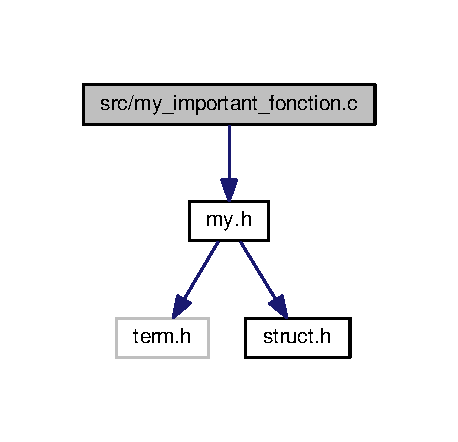
\includegraphics[width=220pt]{my__important__fonction_8c__incl}
\end{center}
\end{figure}
\subsection*{Functions}
\begin{DoxyCompactItemize}
\item 
void \hyperlink{my__important__fonction_8c_a91d6348b48c15f044abee99da6fec6bd}{nothing} ()
\end{DoxyCompactItemize}


\subsection{Function Documentation}
\hypertarget{my__important__fonction_8c_a91d6348b48c15f044abee99da6fec6bd}{\index{my\+\_\+important\+\_\+fonction.\+c@{my\+\_\+important\+\_\+fonction.\+c}!nothing@{nothing}}
\index{nothing@{nothing}!my\+\_\+important\+\_\+fonction.\+c@{my\+\_\+important\+\_\+fonction.\+c}}
\subsubsection[{nothing}]{\setlength{\rightskip}{0pt plus 5cm}void nothing (
\begin{DoxyParamCaption}
{}
\end{DoxyParamCaption}
)}}\label{my__important__fonction_8c_a91d6348b48c15f044abee99da6fec6bd}


Definition at line 13 of file my\+\_\+important\+\_\+fonction.\+c.


\hypertarget{my__move_8c}{\section{src/my\+\_\+move.c File Reference}
\label{my__move_8c}\index{src/my\+\_\+move.\+c@{src/my\+\_\+move.\+c}}
}
{\ttfamily \#include \char`\"{}struct.\+h\char`\"{}}\\*
{\ttfamily \#include \char`\"{}my.\+h\char`\"{}}\\*
Include dependency graph for my\+\_\+move.\+c\+:\nopagebreak
\begin{figure}[H]
\begin{center}
\leavevmode
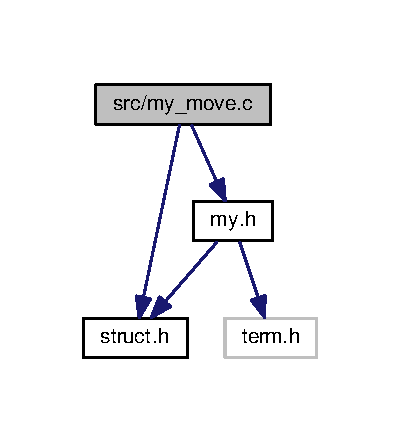
\includegraphics[width=192pt]{my__move_8c__incl}
\end{center}
\end{figure}
\subsection*{Functions}
\begin{DoxyCompactItemize}
\item 
int \hyperlink{my__move_8c_a2451a5c10e20e4b4cb9e0d53bccfcd2a}{case\+\_\+down} (\hyperlink{struct_8h_abb3da8aaebffbf4c0c44fc37b91a41af}{t\+\_\+eta} $\ast$etat)
\item 
int \hyperlink{my__move_8c_a7ed81da7f401ef400973c6f141adac79}{case\+\_\+hight} (\hyperlink{struct_8h_abb3da8aaebffbf4c0c44fc37b91a41af}{t\+\_\+eta} $\ast$etat)
\item 
int \hyperlink{my__move_8c_af686d676ef6348cae9c7ce6de35b6223}{case\+\_\+left} (\hyperlink{struct_8h_abb3da8aaebffbf4c0c44fc37b91a41af}{t\+\_\+eta} $\ast$etat)
\item 
int \hyperlink{my__move_8c_a38fd644159c2b6ce04b987a9a9eb9eb5}{case\+\_\+right} (\hyperlink{struct_8h_abb3da8aaebffbf4c0c44fc37b91a41af}{t\+\_\+eta} $\ast$etat)
\end{DoxyCompactItemize}


\subsection{Function Documentation}
\hypertarget{my__move_8c_a2451a5c10e20e4b4cb9e0d53bccfcd2a}{\index{my\+\_\+move.\+c@{my\+\_\+move.\+c}!case\+\_\+down@{case\+\_\+down}}
\index{case\+\_\+down@{case\+\_\+down}!my\+\_\+move.\+c@{my\+\_\+move.\+c}}
\subsubsection[{case\+\_\+down}]{\setlength{\rightskip}{0pt plus 5cm}int case\+\_\+down (
\begin{DoxyParamCaption}
\item[{{\bf t\+\_\+eta} $\ast$}]{etat}
\end{DoxyParamCaption}
)}}\label{my__move_8c_a2451a5c10e20e4b4cb9e0d53bccfcd2a}


Definition at line 14 of file my\+\_\+move.\+c.

\hypertarget{my__move_8c_a7ed81da7f401ef400973c6f141adac79}{\index{my\+\_\+move.\+c@{my\+\_\+move.\+c}!case\+\_\+hight@{case\+\_\+hight}}
\index{case\+\_\+hight@{case\+\_\+hight}!my\+\_\+move.\+c@{my\+\_\+move.\+c}}
\subsubsection[{case\+\_\+hight}]{\setlength{\rightskip}{0pt plus 5cm}int case\+\_\+hight (
\begin{DoxyParamCaption}
\item[{{\bf t\+\_\+eta} $\ast$}]{etat}
\end{DoxyParamCaption}
)}}\label{my__move_8c_a7ed81da7f401ef400973c6f141adac79}


Definition at line 34 of file my\+\_\+move.\+c.

\hypertarget{my__move_8c_af686d676ef6348cae9c7ce6de35b6223}{\index{my\+\_\+move.\+c@{my\+\_\+move.\+c}!case\+\_\+left@{case\+\_\+left}}
\index{case\+\_\+left@{case\+\_\+left}!my\+\_\+move.\+c@{my\+\_\+move.\+c}}
\subsubsection[{case\+\_\+left}]{\setlength{\rightskip}{0pt plus 5cm}int case\+\_\+left (
\begin{DoxyParamCaption}
\item[{{\bf t\+\_\+eta} $\ast$}]{etat}
\end{DoxyParamCaption}
)}}\label{my__move_8c_af686d676ef6348cae9c7ce6de35b6223}


Definition at line 54 of file my\+\_\+move.\+c.

\hypertarget{my__move_8c_a38fd644159c2b6ce04b987a9a9eb9eb5}{\index{my\+\_\+move.\+c@{my\+\_\+move.\+c}!case\+\_\+right@{case\+\_\+right}}
\index{case\+\_\+right@{case\+\_\+right}!my\+\_\+move.\+c@{my\+\_\+move.\+c}}
\subsubsection[{case\+\_\+right}]{\setlength{\rightskip}{0pt plus 5cm}int case\+\_\+right (
\begin{DoxyParamCaption}
\item[{{\bf t\+\_\+eta} $\ast$}]{etat}
\end{DoxyParamCaption}
)}}\label{my__move_8c_a38fd644159c2b6ce04b987a9a9eb9eb5}


Definition at line 60 of file my\+\_\+move.\+c.


\hypertarget{my__putchar_8c}{\section{src/my\+\_\+putchar.c File Reference}
\label{my__putchar_8c}\index{src/my\+\_\+putchar.\+c@{src/my\+\_\+putchar.\+c}}
}
{\ttfamily \#include $<$unistd.\+h$>$}\\*
{\ttfamily \#include \char`\"{}my.\+h\char`\"{}}\\*
Include dependency graph for my\+\_\+putchar.\+c\+:\nopagebreak
\begin{figure}[H]
\begin{center}
\leavevmode
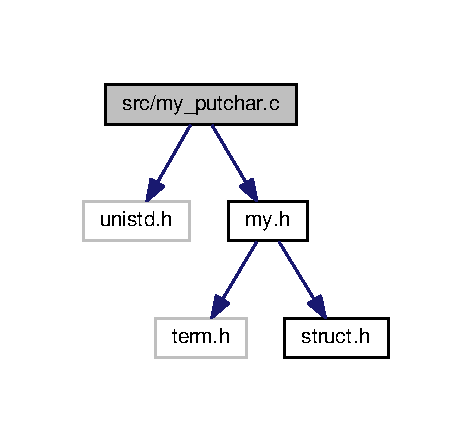
\includegraphics[width=227pt]{my__putchar_8c__incl}
\end{center}
\end{figure}
\subsection*{Functions}
\begin{DoxyCompactItemize}
\item 
void \hyperlink{my__putchar_8c_ac4de74d04dc6e263345755eb62676802}{my\+\_\+putchar} (char c)
\item 
void \hyperlink{my__putchar_8c_ab8c42cc361342e8e3e0e9ff5456ea431}{my\+\_\+putchar\+\_\+fd0} (char c)
\item 
int \hyperlink{my__putchar_8c_ad41a2fc8dcc349d0cc3223eddba3d038}{my\+\_\+putc} (int c)
\end{DoxyCompactItemize}


\subsection{Function Documentation}
\hypertarget{my__putchar_8c_ad41a2fc8dcc349d0cc3223eddba3d038}{\index{my\+\_\+putchar.\+c@{my\+\_\+putchar.\+c}!my\+\_\+putc@{my\+\_\+putc}}
\index{my\+\_\+putc@{my\+\_\+putc}!my\+\_\+putchar.\+c@{my\+\_\+putchar.\+c}}
\subsubsection[{my\+\_\+putc}]{\setlength{\rightskip}{0pt plus 5cm}int my\+\_\+putc (
\begin{DoxyParamCaption}
\item[{int}]{c}
\end{DoxyParamCaption}
)}}\label{my__putchar_8c_ad41a2fc8dcc349d0cc3223eddba3d038}


Definition at line 24 of file my\+\_\+putchar.\+c.

\hypertarget{my__putchar_8c_ac4de74d04dc6e263345755eb62676802}{\index{my\+\_\+putchar.\+c@{my\+\_\+putchar.\+c}!my\+\_\+putchar@{my\+\_\+putchar}}
\index{my\+\_\+putchar@{my\+\_\+putchar}!my\+\_\+putchar.\+c@{my\+\_\+putchar.\+c}}
\subsubsection[{my\+\_\+putchar}]{\setlength{\rightskip}{0pt plus 5cm}void my\+\_\+putchar (
\begin{DoxyParamCaption}
\item[{char}]{c}
\end{DoxyParamCaption}
)}}\label{my__putchar_8c_ac4de74d04dc6e263345755eb62676802}


Definition at line 14 of file my\+\_\+putchar.\+c.

\hypertarget{my__putchar_8c_ab8c42cc361342e8e3e0e9ff5456ea431}{\index{my\+\_\+putchar.\+c@{my\+\_\+putchar.\+c}!my\+\_\+putchar\+\_\+fd0@{my\+\_\+putchar\+\_\+fd0}}
\index{my\+\_\+putchar\+\_\+fd0@{my\+\_\+putchar\+\_\+fd0}!my\+\_\+putchar.\+c@{my\+\_\+putchar.\+c}}
\subsubsection[{my\+\_\+putchar\+\_\+fd0}]{\setlength{\rightskip}{0pt plus 5cm}void my\+\_\+putchar\+\_\+fd0 (
\begin{DoxyParamCaption}
\item[{char}]{c}
\end{DoxyParamCaption}
)}}\label{my__putchar_8c_ab8c42cc361342e8e3e0e9ff5456ea431}


Definition at line 19 of file my\+\_\+putchar.\+c.


\hypertarget{my__putnbr_8c}{\section{src/my\+\_\+putnbr.c File Reference}
\label{my__putnbr_8c}\index{src/my\+\_\+putnbr.\+c@{src/my\+\_\+putnbr.\+c}}
}
{\ttfamily \#include \char`\"{}my.\+h\char`\"{}}\\*
Include dependency graph for my\+\_\+putnbr.\+c\+:\nopagebreak
\begin{figure}[H]
\begin{center}
\leavevmode
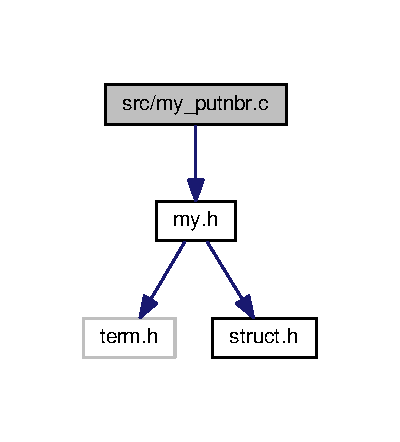
\includegraphics[width=192pt]{my__putnbr_8c__incl}
\end{center}
\end{figure}
\subsection*{Functions}
\begin{DoxyCompactItemize}
\item 
void \hyperlink{my__putnbr_8c_a25366074e11e8eddaa1ba04a2ee13b55}{my\+\_\+putnbr} (int nb)
\end{DoxyCompactItemize}


\subsection{Function Documentation}
\hypertarget{my__putnbr_8c_a25366074e11e8eddaa1ba04a2ee13b55}{\index{my\+\_\+putnbr.\+c@{my\+\_\+putnbr.\+c}!my\+\_\+putnbr@{my\+\_\+putnbr}}
\index{my\+\_\+putnbr@{my\+\_\+putnbr}!my\+\_\+putnbr.\+c@{my\+\_\+putnbr.\+c}}
\subsubsection[{my\+\_\+putnbr}]{\setlength{\rightskip}{0pt plus 5cm}void my\+\_\+putnbr (
\begin{DoxyParamCaption}
\item[{int}]{nb}
\end{DoxyParamCaption}
)}}\label{my__putnbr_8c_a25366074e11e8eddaa1ba04a2ee13b55}


Definition at line 13 of file my\+\_\+putnbr.\+c.


\hypertarget{my__putsterr_8c}{\section{src/my\+\_\+putsterr.c File Reference}
\label{my__putsterr_8c}\index{src/my\+\_\+putsterr.\+c@{src/my\+\_\+putsterr.\+c}}
}
{\ttfamily \#include $<$unistd.\+h$>$}\\*
{\ttfamily \#include $<$stdio.\+h$>$}\\*
{\ttfamily \#include \char`\"{}my.\+h\char`\"{}}\\*
Include dependency graph for my\+\_\+putsterr.\+c\+:\nopagebreak
\begin{figure}[H]
\begin{center}
\leavevmode
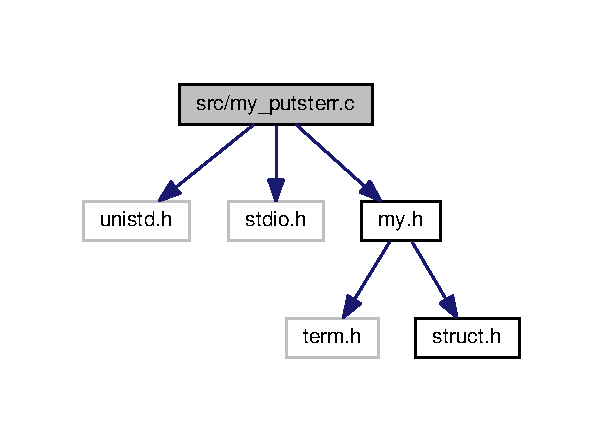
\includegraphics[width=290pt]{my__putsterr_8c__incl}
\end{center}
\end{figure}
\subsection*{Functions}
\begin{DoxyCompactItemize}
\item 
void \hyperlink{my__putsterr_8c_a9167eba68e3185faf9fc9a93c2f30998}{my\+\_\+puterr} (char c)
\item 
void \hyperlink{my__putsterr_8c_abbc8e0d57c6e21f89c3367ece5d6a5c6}{my\+\_\+putsterr} (char $\ast$str)
\end{DoxyCompactItemize}


\subsection{Function Documentation}
\hypertarget{my__putsterr_8c_a9167eba68e3185faf9fc9a93c2f30998}{\index{my\+\_\+putsterr.\+c@{my\+\_\+putsterr.\+c}!my\+\_\+puterr@{my\+\_\+puterr}}
\index{my\+\_\+puterr@{my\+\_\+puterr}!my\+\_\+putsterr.\+c@{my\+\_\+putsterr.\+c}}
\subsubsection[{my\+\_\+puterr}]{\setlength{\rightskip}{0pt plus 5cm}void my\+\_\+puterr (
\begin{DoxyParamCaption}
\item[{char}]{c}
\end{DoxyParamCaption}
)}}\label{my__putsterr_8c_a9167eba68e3185faf9fc9a93c2f30998}


Definition at line 15 of file my\+\_\+putsterr.\+c.

\hypertarget{my__putsterr_8c_abbc8e0d57c6e21f89c3367ece5d6a5c6}{\index{my\+\_\+putsterr.\+c@{my\+\_\+putsterr.\+c}!my\+\_\+putsterr@{my\+\_\+putsterr}}
\index{my\+\_\+putsterr@{my\+\_\+putsterr}!my\+\_\+putsterr.\+c@{my\+\_\+putsterr.\+c}}
\subsubsection[{my\+\_\+putsterr}]{\setlength{\rightskip}{0pt plus 5cm}void my\+\_\+putsterr (
\begin{DoxyParamCaption}
\item[{char $\ast$}]{str}
\end{DoxyParamCaption}
)}}\label{my__putsterr_8c_abbc8e0d57c6e21f89c3367ece5d6a5c6}


Definition at line 20 of file my\+\_\+putsterr.\+c.


\hypertarget{my__putstr_8c}{\section{src/my\+\_\+putstr.c File Reference}
\label{my__putstr_8c}\index{src/my\+\_\+putstr.\+c@{src/my\+\_\+putstr.\+c}}
}
{\ttfamily \#include $<$stdio.\+h$>$}\\*
{\ttfamily \#include \char`\"{}my.\+h\char`\"{}}\\*
Include dependency graph for my\+\_\+putstr.\+c\+:\nopagebreak
\begin{figure}[H]
\begin{center}
\leavevmode
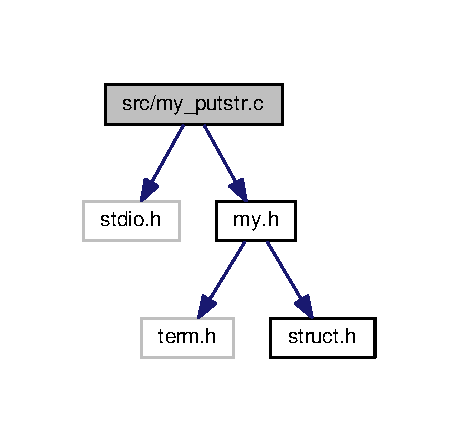
\includegraphics[width=220pt]{my__putstr_8c__incl}
\end{center}
\end{figure}
\subsection*{Functions}
\begin{DoxyCompactItemize}
\item 
void \hyperlink{my__putstr_8c_a90745b48b1811f18086f358dc2b85fd4}{my\+\_\+putstr} (char $\ast$str)
\item 
void \hyperlink{my__putstr_8c_a4dd00910c0d38d20009f91c610e91ec7}{my\+\_\+putstr\+\_\+fd0} (char $\ast$str)
\item 
void \hyperlink{my__putstr_8c_a321389cb2b297d65458e3bc9b80b2410}{my\+\_\+putstr\+\_\+lime} (char $\ast$str, int lime)
\item 
void \hyperlink{my__putstr_8c_a07d17d9593512770b9c6c7d46a6ae5c7}{my\+\_\+put\+\_\+space} (int i)
\end{DoxyCompactItemize}


\subsection{Function Documentation}
\hypertarget{my__putstr_8c_a07d17d9593512770b9c6c7d46a6ae5c7}{\index{my\+\_\+putstr.\+c@{my\+\_\+putstr.\+c}!my\+\_\+put\+\_\+space@{my\+\_\+put\+\_\+space}}
\index{my\+\_\+put\+\_\+space@{my\+\_\+put\+\_\+space}!my\+\_\+putstr.\+c@{my\+\_\+putstr.\+c}}
\subsubsection[{my\+\_\+put\+\_\+space}]{\setlength{\rightskip}{0pt plus 5cm}void my\+\_\+put\+\_\+space (
\begin{DoxyParamCaption}
\item[{int}]{i}
\end{DoxyParamCaption}
)}}\label{my__putstr_8c_a07d17d9593512770b9c6c7d46a6ae5c7}


Definition at line 55 of file my\+\_\+putstr.\+c.

\hypertarget{my__putstr_8c_a90745b48b1811f18086f358dc2b85fd4}{\index{my\+\_\+putstr.\+c@{my\+\_\+putstr.\+c}!my\+\_\+putstr@{my\+\_\+putstr}}
\index{my\+\_\+putstr@{my\+\_\+putstr}!my\+\_\+putstr.\+c@{my\+\_\+putstr.\+c}}
\subsubsection[{my\+\_\+putstr}]{\setlength{\rightskip}{0pt plus 5cm}void my\+\_\+putstr (
\begin{DoxyParamCaption}
\item[{char $\ast$}]{str}
\end{DoxyParamCaption}
)}}\label{my__putstr_8c_a90745b48b1811f18086f358dc2b85fd4}


Definition at line 14 of file my\+\_\+putstr.\+c.

\hypertarget{my__putstr_8c_a4dd00910c0d38d20009f91c610e91ec7}{\index{my\+\_\+putstr.\+c@{my\+\_\+putstr.\+c}!my\+\_\+putstr\+\_\+fd0@{my\+\_\+putstr\+\_\+fd0}}
\index{my\+\_\+putstr\+\_\+fd0@{my\+\_\+putstr\+\_\+fd0}!my\+\_\+putstr.\+c@{my\+\_\+putstr.\+c}}
\subsubsection[{my\+\_\+putstr\+\_\+fd0}]{\setlength{\rightskip}{0pt plus 5cm}void my\+\_\+putstr\+\_\+fd0 (
\begin{DoxyParamCaption}
\item[{char $\ast$}]{str}
\end{DoxyParamCaption}
)}}\label{my__putstr_8c_a4dd00910c0d38d20009f91c610e91ec7}


Definition at line 26 of file my\+\_\+putstr.\+c.

\hypertarget{my__putstr_8c_a321389cb2b297d65458e3bc9b80b2410}{\index{my\+\_\+putstr.\+c@{my\+\_\+putstr.\+c}!my\+\_\+putstr\+\_\+lime@{my\+\_\+putstr\+\_\+lime}}
\index{my\+\_\+putstr\+\_\+lime@{my\+\_\+putstr\+\_\+lime}!my\+\_\+putstr.\+c@{my\+\_\+putstr.\+c}}
\subsubsection[{my\+\_\+putstr\+\_\+lime}]{\setlength{\rightskip}{0pt plus 5cm}void my\+\_\+putstr\+\_\+lime (
\begin{DoxyParamCaption}
\item[{char $\ast$}]{str, }
\item[{int}]{lime}
\end{DoxyParamCaption}
)}}\label{my__putstr_8c_a321389cb2b297d65458e3bc9b80b2410}


Definition at line 38 of file my\+\_\+putstr.\+c.


\hypertarget{my__select_8c}{\section{src/my\+\_\+select.c File Reference}
\label{my__select_8c}\index{src/my\+\_\+select.\+c@{src/my\+\_\+select.\+c}}
}
{\ttfamily \#include $<$stdlib.\+h$>$}\\*
{\ttfamily \#include $<$sys/ioctl.\+h$>$}\\*
{\ttfamily \#include $<$termcap.\+h$>$}\\*
{\ttfamily \#include $<$ncurses/curses.\+h$>$}\\*
{\ttfamily \#include $<$termios.\+h$>$}\\*
{\ttfamily \#include $<$unistd.\+h$>$}\\*
{\ttfamily \#include $<$signal.\+h$>$}\\*
{\ttfamily \#include \char`\"{}struct.\+h\char`\"{}}\\*
{\ttfamily \#include \char`\"{}my.\+h\char`\"{}}\\*
Include dependency graph for my\+\_\+select.\+c\+:\nopagebreak
\begin{figure}[H]
\begin{center}
\leavevmode
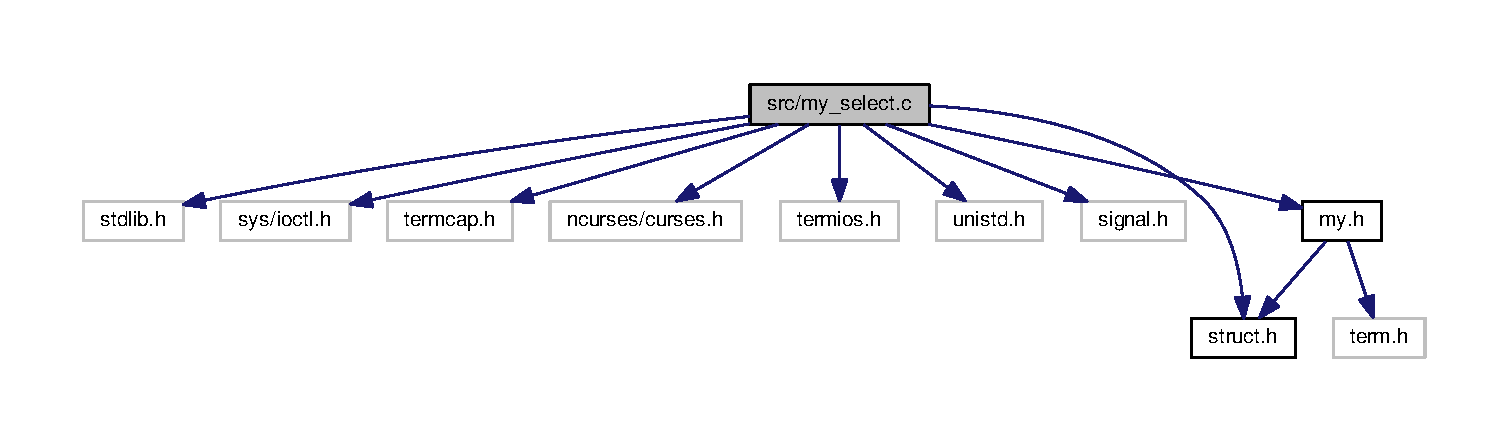
\includegraphics[width=350pt]{my__select_8c__incl}
\end{center}
\end{figure}
\subsection*{Functions}
\begin{DoxyCompactItemize}
\item 
int \hyperlink{my__select_8c_a54107884475937a6a75a9cf11d24a4e2}{my\+\_\+actualisation} (struct termios $\ast$term)
\item 
int \hyperlink{my__select_8c_add91d018cb04acdfb4a5512ca3b19e9d}{my\+\_\+select} (struct termios $\ast$term, \hyperlink{struct_8h_abb3da8aaebffbf4c0c44fc37b91a41af}{t\+\_\+eta} $\ast$etat, int size\+\_\+colone)
\item 
int \hyperlink{my__select_8c_ad868f8855e4adc4512d7212c8705225a}{my\+\_\+gere\+\_\+key} (struct termios $\ast$term, \hyperlink{struct_8h_abb3da8aaebffbf4c0c44fc37b91a41af}{t\+\_\+eta} $\ast$etat)
\item 
int \hyperlink{my__select_8c_a7c31a994c5ec79ecf4144f4ef717112f}{my\+\_\+gere\+\_\+select} (int argc, char $\ast$$\ast$argv, int size\+\_\+colone, struct termios $\ast$term)
\end{DoxyCompactItemize}


\subsection{Function Documentation}
\hypertarget{my__select_8c_a54107884475937a6a75a9cf11d24a4e2}{\index{my\+\_\+select.\+c@{my\+\_\+select.\+c}!my\+\_\+actualisation@{my\+\_\+actualisation}}
\index{my\+\_\+actualisation@{my\+\_\+actualisation}!my\+\_\+select.\+c@{my\+\_\+select.\+c}}
\subsubsection[{my\+\_\+actualisation}]{\setlength{\rightskip}{0pt plus 5cm}int my\+\_\+actualisation (
\begin{DoxyParamCaption}
\item[{struct termios $\ast$}]{term}
\end{DoxyParamCaption}
)}}\label{my__select_8c_a54107884475937a6a75a9cf11d24a4e2}


Definition at line 21 of file my\+\_\+select.\+c.

\hypertarget{my__select_8c_ad868f8855e4adc4512d7212c8705225a}{\index{my\+\_\+select.\+c@{my\+\_\+select.\+c}!my\+\_\+gere\+\_\+key@{my\+\_\+gere\+\_\+key}}
\index{my\+\_\+gere\+\_\+key@{my\+\_\+gere\+\_\+key}!my\+\_\+select.\+c@{my\+\_\+select.\+c}}
\subsubsection[{my\+\_\+gere\+\_\+key}]{\setlength{\rightskip}{0pt plus 5cm}int my\+\_\+gere\+\_\+key (
\begin{DoxyParamCaption}
\item[{struct termios $\ast$}]{term, }
\item[{{\bf t\+\_\+eta} $\ast$}]{etat}
\end{DoxyParamCaption}
)}}\label{my__select_8c_ad868f8855e4adc4512d7212c8705225a}


Definition at line 56 of file my\+\_\+select.\+c.

\hypertarget{my__select_8c_a7c31a994c5ec79ecf4144f4ef717112f}{\index{my\+\_\+select.\+c@{my\+\_\+select.\+c}!my\+\_\+gere\+\_\+select@{my\+\_\+gere\+\_\+select}}
\index{my\+\_\+gere\+\_\+select@{my\+\_\+gere\+\_\+select}!my\+\_\+select.\+c@{my\+\_\+select.\+c}}
\subsubsection[{my\+\_\+gere\+\_\+select}]{\setlength{\rightskip}{0pt plus 5cm}int my\+\_\+gere\+\_\+select (
\begin{DoxyParamCaption}
\item[{int}]{argc, }
\item[{char $\ast$$\ast$}]{argv, }
\item[{int}]{size\+\_\+colone, }
\item[{struct termios $\ast$}]{term}
\end{DoxyParamCaption}
)}}\label{my__select_8c_a7c31a994c5ec79ecf4144f4ef717112f}


Definition at line 80 of file my\+\_\+select.\+c.

\hypertarget{my__select_8c_add91d018cb04acdfb4a5512ca3b19e9d}{\index{my\+\_\+select.\+c@{my\+\_\+select.\+c}!my\+\_\+select@{my\+\_\+select}}
\index{my\+\_\+select@{my\+\_\+select}!my\+\_\+select.\+c@{my\+\_\+select.\+c}}
\subsubsection[{my\+\_\+select}]{\setlength{\rightskip}{0pt plus 5cm}int my\+\_\+select (
\begin{DoxyParamCaption}
\item[{struct termios $\ast$}]{term, }
\item[{{\bf t\+\_\+eta} $\ast$}]{etat, }
\item[{int}]{size\+\_\+colone}
\end{DoxyParamCaption}
)}}\label{my__select_8c_add91d018cb04acdfb4a5512ca3b19e9d}


Definition at line 31 of file my\+\_\+select.\+c.


\hypertarget{my__strlen_8c}{\section{src/my\+\_\+strlen.c File Reference}
\label{my__strlen_8c}\index{src/my\+\_\+strlen.\+c@{src/my\+\_\+strlen.\+c}}
}
{\ttfamily \#include \char`\"{}my.\+h\char`\"{}}\\*
Include dependency graph for my\+\_\+strlen.\+c\+:\nopagebreak
\begin{figure}[H]
\begin{center}
\leavevmode
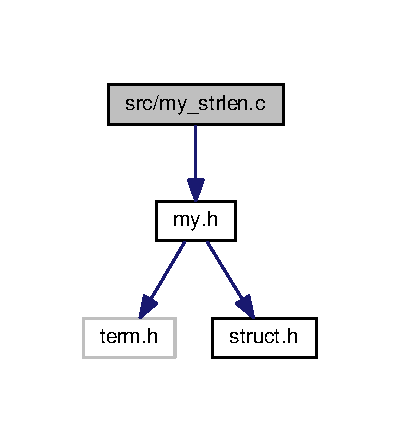
\includegraphics[width=192pt]{my__strlen_8c__incl}
\end{center}
\end{figure}
\subsection*{Functions}
\begin{DoxyCompactItemize}
\item 
int \hyperlink{my__strlen_8c_ac7e9bd08d068851e31a5b6d408004638}{my\+\_\+strlen} (char $\ast$str)
\end{DoxyCompactItemize}


\subsection{Function Documentation}
\hypertarget{my__strlen_8c_ac7e9bd08d068851e31a5b6d408004638}{\index{my\+\_\+strlen.\+c@{my\+\_\+strlen.\+c}!my\+\_\+strlen@{my\+\_\+strlen}}
\index{my\+\_\+strlen@{my\+\_\+strlen}!my\+\_\+strlen.\+c@{my\+\_\+strlen.\+c}}
\subsubsection[{my\+\_\+strlen}]{\setlength{\rightskip}{0pt plus 5cm}int my\+\_\+strlen (
\begin{DoxyParamCaption}
\item[{char $\ast$}]{str}
\end{DoxyParamCaption}
)}}\label{my__strlen_8c_ac7e9bd08d068851e31a5b6d408004638}


Definition at line 13 of file my\+\_\+strlen.\+c.


\hypertarget{struct_8h}{\section{src/struct.h File Reference}
\label{struct_8h}\index{src/struct.\+h@{src/struct.\+h}}
}
This graph shows which files directly or indirectly include this file\+:\nopagebreak
\begin{figure}[H]
\begin{center}
\leavevmode
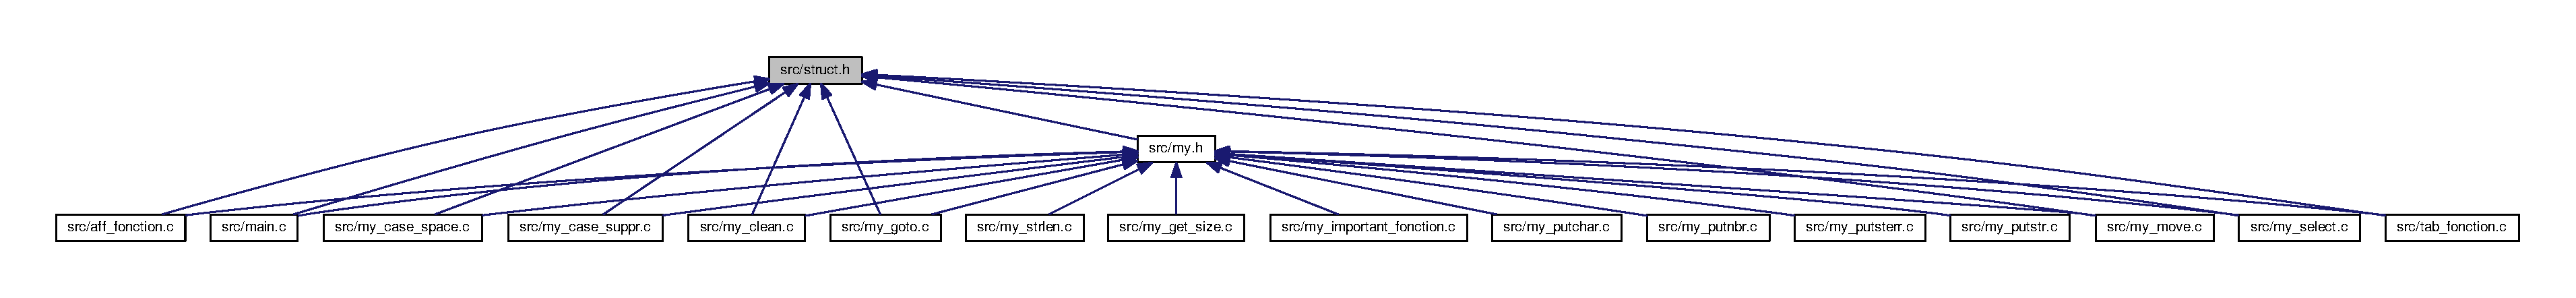
\includegraphics[width=350pt]{struct_8h__dep__incl}
\end{center}
\end{figure}
\subsection*{Data Structures}
\begin{DoxyCompactItemize}
\item 
struct \hyperlink{structs__win}{s\+\_\+win}
\item 
struct \hyperlink{structs__eta}{s\+\_\+eta}
\item 
struct \hyperlink{structs__key}{s\+\_\+key}
\end{DoxyCompactItemize}
\subsection*{Macros}
\begin{DoxyCompactItemize}
\item 
\#define \hyperlink{struct_8h_a3cdca3262c81fd4c287fa6f4807167c4}{H\+I\+G\+H\+T}~4283163
\item 
\#define \hyperlink{struct_8h_a4193cd1c8c2e6ebd0e056fa2364a663f}{D\+O\+W\+N}~4348699
\item 
\#define \hyperlink{struct_8h_a437ef08681e7210d6678427030446a54}{L\+E\+F\+T}~4479771
\item 
\#define \hyperlink{struct_8h_a80fb826a684cf3f0d306b22aa100ddac}{R\+I\+G\+H\+T}~4414235
\item 
\#define \hyperlink{struct_8h_a4af1b6159e447ba72652bb7fcdfa726e}{E\+S\+C}~27
\item 
\#define \hyperlink{struct_8h_a5ff6e798033f03e74730e99f01936f84}{S\+P\+A\+C\+E}~32
\item 
\#define \hyperlink{struct_8h_a9dba8e1e667dc0da64c02c196b750a7a}{E\+N\+T}~10
\item 
\#define \hyperlink{struct_8h_ad8c54f10d660e17b86fbea8681298d17}{S\+U\+P\+P\+R\+\_\+\+K\+E\+Y}~127
\item 
\#define \hyperlink{struct_8h_aadcd61c629dac0c25f793abb2d0cd77d}{S\+U\+P\+P\+R\+\_\+\+S\+Y\+S\+T}~1741551364
\end{DoxyCompactItemize}
\subsection*{Typedefs}
\begin{DoxyCompactItemize}
\item 
typedef struct \hyperlink{structs__win}{s\+\_\+win} \hyperlink{struct_8h_a926b4cd56a88892e139db39d72aa5753}{t\+\_\+win}
\item 
typedef struct \hyperlink{structs__eta}{s\+\_\+eta} \hyperlink{struct_8h_abb3da8aaebffbf4c0c44fc37b91a41af}{t\+\_\+eta}
\item 
typedef struct \hyperlink{structs__key}{s\+\_\+key} \hyperlink{struct_8h_aca9dc3aa395d996f001d58f70e11a70d}{t\+\_\+key}
\end{DoxyCompactItemize}


\subsection{Macro Definition Documentation}
\hypertarget{struct_8h_a4193cd1c8c2e6ebd0e056fa2364a663f}{\index{struct.\+h@{struct.\+h}!D\+O\+W\+N@{D\+O\+W\+N}}
\index{D\+O\+W\+N@{D\+O\+W\+N}!struct.\+h@{struct.\+h}}
\subsubsection[{D\+O\+W\+N}]{\setlength{\rightskip}{0pt plus 5cm}\#define D\+O\+W\+N~4348699}}\label{struct_8h_a4193cd1c8c2e6ebd0e056fa2364a663f}


Definition at line 15 of file struct.\+h.

\hypertarget{struct_8h_a9dba8e1e667dc0da64c02c196b750a7a}{\index{struct.\+h@{struct.\+h}!E\+N\+T@{E\+N\+T}}
\index{E\+N\+T@{E\+N\+T}!struct.\+h@{struct.\+h}}
\subsubsection[{E\+N\+T}]{\setlength{\rightskip}{0pt plus 5cm}\#define E\+N\+T~10}}\label{struct_8h_a9dba8e1e667dc0da64c02c196b750a7a}


Definition at line 20 of file struct.\+h.

\hypertarget{struct_8h_a4af1b6159e447ba72652bb7fcdfa726e}{\index{struct.\+h@{struct.\+h}!E\+S\+C@{E\+S\+C}}
\index{E\+S\+C@{E\+S\+C}!struct.\+h@{struct.\+h}}
\subsubsection[{E\+S\+C}]{\setlength{\rightskip}{0pt plus 5cm}\#define E\+S\+C~27}}\label{struct_8h_a4af1b6159e447ba72652bb7fcdfa726e}


Definition at line 18 of file struct.\+h.

\hypertarget{struct_8h_a3cdca3262c81fd4c287fa6f4807167c4}{\index{struct.\+h@{struct.\+h}!H\+I\+G\+H\+T@{H\+I\+G\+H\+T}}
\index{H\+I\+G\+H\+T@{H\+I\+G\+H\+T}!struct.\+h@{struct.\+h}}
\subsubsection[{H\+I\+G\+H\+T}]{\setlength{\rightskip}{0pt plus 5cm}\#define H\+I\+G\+H\+T~4283163}}\label{struct_8h_a3cdca3262c81fd4c287fa6f4807167c4}


Definition at line 14 of file struct.\+h.

\hypertarget{struct_8h_a437ef08681e7210d6678427030446a54}{\index{struct.\+h@{struct.\+h}!L\+E\+F\+T@{L\+E\+F\+T}}
\index{L\+E\+F\+T@{L\+E\+F\+T}!struct.\+h@{struct.\+h}}
\subsubsection[{L\+E\+F\+T}]{\setlength{\rightskip}{0pt plus 5cm}\#define L\+E\+F\+T~4479771}}\label{struct_8h_a437ef08681e7210d6678427030446a54}


Definition at line 16 of file struct.\+h.

\hypertarget{struct_8h_a80fb826a684cf3f0d306b22aa100ddac}{\index{struct.\+h@{struct.\+h}!R\+I\+G\+H\+T@{R\+I\+G\+H\+T}}
\index{R\+I\+G\+H\+T@{R\+I\+G\+H\+T}!struct.\+h@{struct.\+h}}
\subsubsection[{R\+I\+G\+H\+T}]{\setlength{\rightskip}{0pt plus 5cm}\#define R\+I\+G\+H\+T~4414235}}\label{struct_8h_a80fb826a684cf3f0d306b22aa100ddac}


Definition at line 17 of file struct.\+h.

\hypertarget{struct_8h_a5ff6e798033f03e74730e99f01936f84}{\index{struct.\+h@{struct.\+h}!S\+P\+A\+C\+E@{S\+P\+A\+C\+E}}
\index{S\+P\+A\+C\+E@{S\+P\+A\+C\+E}!struct.\+h@{struct.\+h}}
\subsubsection[{S\+P\+A\+C\+E}]{\setlength{\rightskip}{0pt plus 5cm}\#define S\+P\+A\+C\+E~32}}\label{struct_8h_a5ff6e798033f03e74730e99f01936f84}


Definition at line 19 of file struct.\+h.

\hypertarget{struct_8h_ad8c54f10d660e17b86fbea8681298d17}{\index{struct.\+h@{struct.\+h}!S\+U\+P\+P\+R\+\_\+\+K\+E\+Y@{S\+U\+P\+P\+R\+\_\+\+K\+E\+Y}}
\index{S\+U\+P\+P\+R\+\_\+\+K\+E\+Y@{S\+U\+P\+P\+R\+\_\+\+K\+E\+Y}!struct.\+h@{struct.\+h}}
\subsubsection[{S\+U\+P\+P\+R\+\_\+\+K\+E\+Y}]{\setlength{\rightskip}{0pt plus 5cm}\#define S\+U\+P\+P\+R\+\_\+\+K\+E\+Y~127}}\label{struct_8h_ad8c54f10d660e17b86fbea8681298d17}


Definition at line 21 of file struct.\+h.

\hypertarget{struct_8h_aadcd61c629dac0c25f793abb2d0cd77d}{\index{struct.\+h@{struct.\+h}!S\+U\+P\+P\+R\+\_\+\+S\+Y\+S\+T@{S\+U\+P\+P\+R\+\_\+\+S\+Y\+S\+T}}
\index{S\+U\+P\+P\+R\+\_\+\+S\+Y\+S\+T@{S\+U\+P\+P\+R\+\_\+\+S\+Y\+S\+T}!struct.\+h@{struct.\+h}}
\subsubsection[{S\+U\+P\+P\+R\+\_\+\+S\+Y\+S\+T}]{\setlength{\rightskip}{0pt plus 5cm}\#define S\+U\+P\+P\+R\+\_\+\+S\+Y\+S\+T~1741551364}}\label{struct_8h_aadcd61c629dac0c25f793abb2d0cd77d}


Definition at line 22 of file struct.\+h.



\subsection{Typedef Documentation}
\hypertarget{struct_8h_abb3da8aaebffbf4c0c44fc37b91a41af}{\index{struct.\+h@{struct.\+h}!t\+\_\+eta@{t\+\_\+eta}}
\index{t\+\_\+eta@{t\+\_\+eta}!struct.\+h@{struct.\+h}}
\subsubsection[{t\+\_\+eta}]{\setlength{\rightskip}{0pt plus 5cm}typedef struct {\bf s\+\_\+eta}			 {\bf t\+\_\+eta}}}\label{struct_8h_abb3da8aaebffbf4c0c44fc37b91a41af}
\hypertarget{struct_8h_aca9dc3aa395d996f001d58f70e11a70d}{\index{struct.\+h@{struct.\+h}!t\+\_\+key@{t\+\_\+key}}
\index{t\+\_\+key@{t\+\_\+key}!struct.\+h@{struct.\+h}}
\subsubsection[{t\+\_\+key}]{\setlength{\rightskip}{0pt plus 5cm}typedef struct {\bf s\+\_\+key}			 {\bf t\+\_\+key}}}\label{struct_8h_aca9dc3aa395d996f001d58f70e11a70d}
\hypertarget{struct_8h_a926b4cd56a88892e139db39d72aa5753}{\index{struct.\+h@{struct.\+h}!t\+\_\+win@{t\+\_\+win}}
\index{t\+\_\+win@{t\+\_\+win}!struct.\+h@{struct.\+h}}
\subsubsection[{t\+\_\+win}]{\setlength{\rightskip}{0pt plus 5cm}typedef struct {\bf s\+\_\+win}			 {\bf t\+\_\+win}}}\label{struct_8h_a926b4cd56a88892e139db39d72aa5753}

\hypertarget{tab__fonction_8c}{\section{src/tab\+\_\+fonction.c File Reference}
\label{tab__fonction_8c}\index{src/tab\+\_\+fonction.\+c@{src/tab\+\_\+fonction.\+c}}
}
{\ttfamily \#include \char`\"{}my.\+h\char`\"{}}\\*
{\ttfamily \#include \char`\"{}struct.\+h\char`\"{}}\\*
Include dependency graph for tab\+\_\+fonction.\+c\+:\nopagebreak
\begin{figure}[H]
\begin{center}
\leavevmode
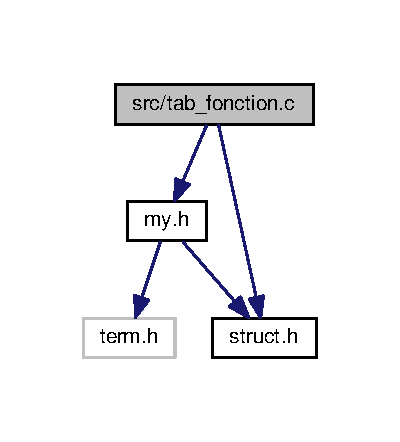
\includegraphics[width=192pt]{tab__fonction_8c__incl}
\end{center}
\end{figure}
\subsection*{Functions}
\begin{DoxyCompactItemize}
\item 
void \hyperlink{tab__fonction_8c_ac787a46c22238927aeccb015549de725}{my\+\_\+init\+\_\+tab} (\hyperlink{struct_8h_abb3da8aaebffbf4c0c44fc37b91a41af}{t\+\_\+eta} $\ast$etat, int argc, char $\ast$$\ast$argv)
\item 
int \hyperlink{tab__fonction_8c_aeaf66e886e7b245a2b3dece3103f2a66}{my\+\_\+ptr\+\_\+tab} (unsigned long buffer, \hyperlink{struct_8h_abb3da8aaebffbf4c0c44fc37b91a41af}{t\+\_\+eta} $\ast$etat)
\item 
void \hyperlink{tab__fonction_8c_a72df070a1ab4704b8545b03005769b19}{my\+\_\+show\+\_\+tab} (\hyperlink{struct_8h_abb3da8aaebffbf4c0c44fc37b91a41af}{t\+\_\+eta} $\ast$etat, \hyperlink{struct_8h_a926b4cd56a88892e139db39d72aa5753}{t\+\_\+win} $\ast$win, int size\+\_\+colone)
\end{DoxyCompactItemize}


\subsection{Function Documentation}
\hypertarget{tab__fonction_8c_ac787a46c22238927aeccb015549de725}{\index{tab\+\_\+fonction.\+c@{tab\+\_\+fonction.\+c}!my\+\_\+init\+\_\+tab@{my\+\_\+init\+\_\+tab}}
\index{my\+\_\+init\+\_\+tab@{my\+\_\+init\+\_\+tab}!tab\+\_\+fonction.\+c@{tab\+\_\+fonction.\+c}}
\subsubsection[{my\+\_\+init\+\_\+tab}]{\setlength{\rightskip}{0pt plus 5cm}void my\+\_\+init\+\_\+tab (
\begin{DoxyParamCaption}
\item[{{\bf t\+\_\+eta} $\ast$}]{etat, }
\item[{int}]{argc, }
\item[{char $\ast$$\ast$}]{argv}
\end{DoxyParamCaption}
)}}\label{tab__fonction_8c_ac787a46c22238927aeccb015549de725}


Definition at line 14 of file tab\+\_\+fonction.\+c.

\hypertarget{tab__fonction_8c_aeaf66e886e7b245a2b3dece3103f2a66}{\index{tab\+\_\+fonction.\+c@{tab\+\_\+fonction.\+c}!my\+\_\+ptr\+\_\+tab@{my\+\_\+ptr\+\_\+tab}}
\index{my\+\_\+ptr\+\_\+tab@{my\+\_\+ptr\+\_\+tab}!tab\+\_\+fonction.\+c@{tab\+\_\+fonction.\+c}}
\subsubsection[{my\+\_\+ptr\+\_\+tab}]{\setlength{\rightskip}{0pt plus 5cm}int my\+\_\+ptr\+\_\+tab (
\begin{DoxyParamCaption}
\item[{unsigned long}]{buffer, }
\item[{{\bf t\+\_\+eta} $\ast$}]{etat}
\end{DoxyParamCaption}
)}}\label{tab__fonction_8c_aeaf66e886e7b245a2b3dece3103f2a66}


Definition at line 33 of file tab\+\_\+fonction.\+c.

\hypertarget{tab__fonction_8c_a72df070a1ab4704b8545b03005769b19}{\index{tab\+\_\+fonction.\+c@{tab\+\_\+fonction.\+c}!my\+\_\+show\+\_\+tab@{my\+\_\+show\+\_\+tab}}
\index{my\+\_\+show\+\_\+tab@{my\+\_\+show\+\_\+tab}!tab\+\_\+fonction.\+c@{tab\+\_\+fonction.\+c}}
\subsubsection[{my\+\_\+show\+\_\+tab}]{\setlength{\rightskip}{0pt plus 5cm}void my\+\_\+show\+\_\+tab (
\begin{DoxyParamCaption}
\item[{{\bf t\+\_\+eta} $\ast$}]{etat, }
\item[{{\bf t\+\_\+win} $\ast$}]{win, }
\item[{int}]{size\+\_\+colone}
\end{DoxyParamCaption}
)}}\label{tab__fonction_8c_a72df070a1ab4704b8545b03005769b19}


Definition at line 54 of file tab\+\_\+fonction.\+c.


%--- End generated contents ---

% Index
\newpage
\phantomsection
\addcontentsline{toc}{chapter}{Index}
\printindex

\end{document}
